\documentclass[12pt, openany, oneside]{book}

\usepackage{tikz}
\usepackage{float}
\usepackage{pgfplots}

\usepgfplotslibrary{fillbetween}

\pgfplotsset{every axis/.append style={
    axis x line=middle,
    axis y line=middle,
    axis line style={->},
}}

%%%%%%%%%%%%%%%%%%%%%%%%%%%%%%%%%%%%%%%%%
% The Legrand Orange Book
% Structural Definitions File
% Version 2.1 (26/09/2018)
%
% Original author:
% Mathias Legrand (legrand.mathias@gmail.com) with modifications by:
% Vel (vel@latextemplates.com)
% 
% This file was downloaded from:
% http://www.LaTeXTemplates.com
%
% License:
% CC BY-NC-SA 3.0 (http://creativecommons.org/licenses/by-nc-sa/3.0/)
%
%%%%%%%%%%%%%%%%%%%%%%%%%%%%%%%%%%%%%%%%%

%----------------------------------------------------------------------------------------
%	VARIOUS REQUIRED PACKAGES AND CONFIGURATIONS
%----------------------------------------------------------------------------------------

\usepackage{graphicx} % Required for including pictures
\graphicspath{{Pictures/}} % Specifies the directory where pictures are stored

\usepackage{lipsum} % Inserts dummy text

\usepackage{tikz} % Required for drawing custom shapes

\usepackage[english]{babel} % English language/hyphenation

\usepackage{enumitem} % Customize lists
\setlist{nolistsep} % Reduce spacing between bullet points and numbered lists

\usepackage{booktabs} % Required for nicer horizontal rules in tables

\usepackage{xcolor} % Required for specifying colors by name
\definecolor{ocre}{RGB}{243,102,25} % Define the orange color used for highlighting throughout the book

%----------------------------------------------------------------------------------------
%	MARGINS
%----------------------------------------------------------------------------------------

\usepackage{geometry} % Required for adjusting page dimensions and margins

\geometry{
	paper=a4paper, % Paper size, change to letterpaper for US letter size
	top=3cm, % Top margin
	bottom=3cm, % Bottom margin
	left=3cm, % Left margin
	right=3cm, % Right margin
	headheight=14pt, % Header height
	footskip=1.4cm, % Space from the bottom margin to the baseline of the footer
	headsep=10pt, % Space from the top margin to the baseline of the header
	%showframe, % Uncomment to show how the type block is set on the page
}

%----------------------------------------------------------------------------------------
%	FONTS
%----------------------------------------------------------------------------------------

\usepackage{avant} % Use the Avantgarde font for headings
%\usepackage{times} % Use the Times font for headings
\usepackage{mathptmx} % Use the Adobe Times Roman as the default text font together with math symbols from the Sym­bol, Chancery and Com­puter Modern fonts

\usepackage{microtype} % Slightly tweak font spacing for aesthetics
\usepackage[utf8]{inputenc} % Required for including letters with accents
\usepackage[T1]{fontenc} % Use 8-bit encoding that has 256 glyphs

%----------------------------------------------------------------------------------------
%	BIBLIOGRAPHY AND INDEX
%----------------------------------------------------------------------------------------

\usepackage[style=numeric,citestyle=numeric,sorting=nyt,sortcites=true,autopunct=true,babel=hyphen,hyperref=true,abbreviate=false,backref=true,backend=biber]{biblatex}
\addbibresource{bibliography.bib} % BibTeX bibliography file
\defbibheading{bibempty}{}

\usepackage{calc} % For simpler calculation - used for spacing the index letter headings correctly
\usepackage{makeidx} % Required to make an index
\makeindex % Tells LaTeX to create the files required for indexing

%----------------------------------------------------------------------------------------
%	MAIN TABLE OF CONTENTS
%----------------------------------------------------------------------------------------

\usepackage{titletoc} % Required for manipulating the table of contents

\contentsmargin{0cm} % Removes the default margin

% Part text styling (this is mostly taken care of in the PART HEADINGS section of this file)
\titlecontents{part}
	[0cm] % Left indentation
	{\addvspace{20pt}\bfseries} % Spacing and font options for parts
	{}
	{}
	{}

% Chapter text styling
\titlecontents{chapter}
	[1.25cm] % Left indentation
	{\addvspace{12pt}\large\sffamily\bfseries} % Spacing and font options for chapters
	{\color{ocre!60}\contentslabel[\Large\thecontentslabel]{1.25cm}\color{ocre}} % Formatting of numbered sections of this type
	{\color{ocre}} % Formatting of numberless sections of this type
	{\color{ocre!60}\normalsize\;\titlerule*[.5pc]{.}\;\thecontentspage} % Formatting of the filler to the right of the heading and the page number

% Section text styling
\titlecontents{section}
	[1.25cm] % Left indentation
	{\addvspace{3pt}\sffamily\bfseries} % Spacing and font options for sections
	{\contentslabel[\thecontentslabel]{1.25cm}} % Formatting of numbered sections of this type
	{} % Formatting of numberless sections of this type
	{\hfill\color{black}\thecontentspage} % Formatting of the filler to the right of the heading and the page number

% Subsection text styling
\titlecontents{subsection}
	[1.25cm] % Left indentation
	{\addvspace{1pt}\sffamily\small} % Spacing and font options for subsections
	{\contentslabel[\thecontentslabel]{1.25cm}} % Formatting of numbered sections of this type
	{} % Formatting of numberless sections of this type
	{\ \titlerule*[.5pc]{.}\;\thecontentspage} % Formatting of the filler to the right of the heading and the page number

% Figure text styling
\titlecontents{figure}
	[1.25cm] % Left indentation
	{\addvspace{1pt}\sffamily\small} % Spacing and font options for figures
	{\thecontentslabel\hspace*{1em}} % Formatting of numbered sections of this type
	{} % Formatting of numberless sections of this type
	{\ \titlerule*[.5pc]{.}\;\thecontentspage} % Formatting of the filler to the right of the heading and the page number

% Table text styling
\titlecontents{table}
	[1.25cm] % Left indentation
	{\addvspace{1pt}\sffamily\small} % Spacing and font options for tables
	{\thecontentslabel\hspace*{1em}} % Formatting of numbered sections of this type
	{} % Formatting of numberless sections of this type
	{\ \titlerule*[.5pc]{.}\;\thecontentspage} % Formatting of the filler to the right of the heading and the page number

%----------------------------------------------------------------------------------------
%	MINI TABLE OF CONTENTS IN PART HEADS
%----------------------------------------------------------------------------------------

% Chapter text styling
\titlecontents{lchapter}
	[0em] % Left indentation
	{\addvspace{15pt}\large\sffamily\bfseries} % Spacing and font options for chapters
	{\color{ocre}\contentslabel[\Large\thecontentslabel]{1.25cm}\color{ocre}} % Chapter number
	{}  
	{\color{ocre}\normalsize\sffamily\bfseries\;\titlerule*[.5pc]{.}\;\thecontentspage} % Page number

% Section text styling
\titlecontents{lsection}
	[0em] % Left indentation
	{\sffamily\small} % Spacing and font options for sections
	{\contentslabel[\thecontentslabel]{1.25cm}} % Section number
	{}
	{}

% Subsection text styling (note these aren't shown by default, display them by searchings this file for tocdepth and reading the commented text)
\titlecontents{lsubsection}
	[.5em] % Left indentation
	{\sffamily\footnotesize} % Spacing and font options for subsections
	{\contentslabel[\thecontentslabel]{1.25cm}}
	{}
	{}

%----------------------------------------------------------------------------------------
%	HEADERS AND FOOTERS
%----------------------------------------------------------------------------------------

\usepackage{fancyhdr} % Required for header and footer configuration

\pagestyle{fancy} % Enable the custom headers and footers

\renewcommand{\chaptermark}[1]{\markboth{\sffamily\normalsize\bfseries\chaptername\ \thechapter.\ #1}{}} % Styling for the current chapter in the header
\renewcommand{\sectionmark}[1]{\markright{\sffamily\normalsize\thesection\hspace{5pt}#1}{}} % Styling for the current section in the header

\fancyhf{} % Clear default headers and footers
\fancyhead[LE,RO]{\sffamily\normalsize\thepage} % Styling for the page number in the header
\fancyhead[LO]{\rightmark} % Print the nearest section name on the left side of odd pages
\fancyhead[RE]{\leftmark} % Print the current chapter name on the right side of even pages
%\fancyfoot[C]{\thepage} % Uncomment to include a footer

\renewcommand{\headrulewidth}{0.5pt} % Thickness of the rule under the header

\fancypagestyle{plain}{% Style for when a plain pagestyle is specified
	\fancyhead{}\renewcommand{\headrulewidth}{0pt}%
}

% Removes the header from odd empty pages at the end of chapters
\makeatletter
\renewcommand{\cleardoublepage}{
\clearpage\ifodd\c@page\else
\hbox{}
\vspace*{\fill}
\thispagestyle{empty}
\newpage
\fi}

%----------------------------------------------------------------------------------------
%	THEOREM STYLES
%----------------------------------------------------------------------------------------

\usepackage{amsmath,amsfonts,amssymb,amsthm} % For math equations, theorems, symbols, etc

\newcommand{\intoo}[2]{\mathopen{]}#1\,;#2\mathclose{[}}
\newcommand{\ud}{\mathop{\mathrm{{}d}}\mathopen{}}
\newcommand{\intff}[2]{\mathopen{[}#1\,;#2\mathclose{]}}
\renewcommand{\qedsymbol}{$\blacksquare$}
\newtheorem{notation}{Notation}[chapter]

% Boxed/framed environments
\newtheoremstyle{ocrenumbox}% Theorem style name
{0pt}% Space above
{0pt}% Space below
{\normalfont}% Body font
{}% Indent amount
{\small\bf\sffamily\color{ocre}}% Theorem head font
{\;}% Punctuation after theorem head
{0.25em}% Space after theorem head
{\small\sffamily\color{ocre}\thmname{#1}\nobreakspace\thmnumber{\@ifnotempty{#1}{}\@upn{#2}}% Theorem text (e.g. Theorem 2.1)
\thmnote{\nobreakspace\the\thm@notefont\sffamily\bfseries\color{black}---\nobreakspace#3.}} % Optional theorem note

\newtheoremstyle{blacknumex}% Theorem style name
{5pt}% Space above
{5pt}% Space below
{\normalfont}% Body font
{} % Indent amount
{\small\bf\sffamily}% Theorem head font
{\;}% Punctuation after theorem head
{0.25em}% Space after theorem head
{\small\sffamily{\tiny\ensuremath{\blacksquare}}\nobreakspace\thmname{#1}\nobreakspace\thmnumber{\@ifnotempty{#1}{}\@upn{#2}}% Theorem text (e.g. Theorem 2.1)
\thmnote{\nobreakspace\the\thm@notefont\sffamily\bfseries---\nobreakspace#3.}}% Optional theorem note

\newtheoremstyle{blacknumbox} % Theorem style name
{0pt}% Space above
{0pt}% Space below
{\normalfont}% Body font
{}% Indent amount
{\small\bf\sffamily}% Theorem head font
{\;}% Punctuation after theorem head
{0.25em}% Space after theorem head
{\small\sffamily\thmname{#1}\nobreakspace\thmnumber{\@ifnotempty{#1}{}\@upn{#2}}% Theorem text (e.g. Theorem 2.1)
\thmnote{\nobreakspace\the\thm@notefont\sffamily\bfseries---\nobreakspace#3.}}% Optional theorem note

% Non-boxed/non-framed environments
\newtheoremstyle{ocrenum}% Theorem style name
{5pt}% Space above
{5pt}% Space below
{\normalfont}% Body font
{}% Indent amount
{\small\bf\sffamily\color{ocre}}% Theorem head font
{\;}% Punctuation after theorem head
{0.25em}% Space after theorem head
{\small\sffamily\color{ocre}\thmname{#1}\nobreakspace\thmnumber{\@ifnotempty{#1}{}\@upn{#2}}% Theorem text (e.g. Theorem 2.1)
\thmnote{\nobreakspace\the\thm@notefont\sffamily\bfseries\color{black}---\nobreakspace#3.}} % Optional theorem note
\makeatother

% Defines the theorem text style for each type of theorem to one of the three styles above
\newcounter{dummy} 
\numberwithin{dummy}{section}
\theoremstyle{ocrenumbox}
\newtheorem{theoremeT}[dummy]{Theorem}
\newtheorem{problem}{Problem}[chapter]
\newtheorem{exerciseT}{Exercise}[chapter]
\theoremstyle{blacknumex}
\newtheorem{exampleT}{Example}[chapter]
\theoremstyle{blacknumbox}
\newtheorem{vocabulary}{Vocabulary}[chapter]
\newtheorem{definitionT}{Definition}[section]
\newtheorem{corollaryT}[dummy]{Corollary}
\theoremstyle{ocrenum}
\newtheorem{proposition}[dummy]{Proposition}

%----------------------------------------------------------------------------------------
%	DEFINITION OF COLORED BOXES
%----------------------------------------------------------------------------------------

\RequirePackage[framemethod=default]{mdframed} % Required for creating the theorem, definition, exercise and corollary boxes

% Theorem box
\newmdenv[skipabove=7pt,
skipbelow=7pt,
backgroundcolor=black!5,
linecolor=ocre,
innerleftmargin=5pt,
innerrightmargin=5pt,
innertopmargin=5pt,
leftmargin=0cm,
rightmargin=0cm,
innerbottommargin=5pt]{tBox}

% Exercise box	  
\newmdenv[skipabove=7pt,
skipbelow=7pt,
rightline=false,
leftline=true,
topline=false,
bottomline=false,
backgroundcolor=ocre!10,
linecolor=ocre,
innerleftmargin=5pt,
innerrightmargin=5pt,
innertopmargin=5pt,
innerbottommargin=5pt,
leftmargin=0cm,
rightmargin=0cm,
linewidth=4pt]{eBox}	

% Definition box
\newmdenv[skipabove=7pt,
skipbelow=7pt,
rightline=false,
leftline=true,
topline=false,
bottomline=false,
linecolor=ocre,
innerleftmargin=5pt,
innerrightmargin=5pt,
innertopmargin=0pt,
leftmargin=0cm,
rightmargin=0cm,
linewidth=4pt,
innerbottommargin=0pt]{dBox}	

% Corollary box
\newmdenv[skipabove=7pt,
skipbelow=7pt,
rightline=false,
leftline=true,
topline=false,
bottomline=false,
linecolor=gray,
backgroundcolor=black!5,
innerleftmargin=5pt,
innerrightmargin=5pt,
innertopmargin=5pt,
leftmargin=0cm,
rightmargin=0cm,
linewidth=4pt,
innerbottommargin=5pt]{cBox}

% Creates an environment for each type of theorem and assigns it a theorem text style from the "Theorem Styles" section above and a colored box from above
\newenvironment{theorem}{\begin{tBox}\begin{theoremeT}}{\end{theoremeT}\end{tBox}}
\newenvironment{exercise}{\begin{eBox}\begin{exerciseT}}{\hfill{\color{ocre}\tiny\ensuremath{\blacksquare}}\end{exerciseT}\end{eBox}}				  
\newenvironment{definition}{\begin{dBox}\begin{definitionT}}{\end{definitionT}\end{dBox}}	
\newenvironment{example}{\begin{exampleT}}{\hfill{\tiny\ensuremath{\blacksquare}}\end{exampleT}}		
\newenvironment{corollary}{\begin{cBox}\begin{corollaryT}}{\end{corollaryT}\end{cBox}}	

%----------------------------------------------------------------------------------------
%	REMARK ENVIRONMENT
%----------------------------------------------------------------------------------------

\newenvironment{remark}{\par\vspace{10pt}\small % Vertical white space above the remark and smaller font size
\begin{list}{}{
\leftmargin=35pt % Indentation on the left
\rightmargin=25pt}\item\ignorespaces % Indentation on the right
\makebox[-2.5pt]{\begin{tikzpicture}[overlay]
\node[draw=ocre!60,line width=1pt,circle,fill=ocre!25,font=\sffamily\bfseries,inner sep=2pt,outer sep=0pt] at (-15pt,0pt){\textcolor{ocre}{R}};\end{tikzpicture}} % Orange R in a circle
\advance\baselineskip -1pt}{\end{list}\vskip5pt} % Tighter line spacing and white space after remark

%----------------------------------------------------------------------------------------
%	SECTION NUMBERING IN THE MARGIN
%----------------------------------------------------------------------------------------

\makeatletter
\renewcommand{\@seccntformat}[1]{\llap{\textcolor{ocre}{\csname the#1\endcsname}\hspace{1em}}}                    
\renewcommand{\section}{\@startsection{section}{1}{\z@}
{-4ex \@plus -1ex \@minus -.4ex}
{1ex \@plus.2ex }
{\normalfont\large\sffamily\bfseries}}
\renewcommand{\subsection}{\@startsection {subsection}{2}{\z@}
{-3ex \@plus -0.1ex \@minus -.4ex}
{0.5ex \@plus.2ex }
{\normalfont\sffamily\bfseries}}
\renewcommand{\subsubsection}{\@startsection {subsubsection}{3}{\z@}
{-2ex \@plus -0.1ex \@minus -.2ex}
{.2ex \@plus.2ex }
{\normalfont\small\sffamily\bfseries}}                        
\renewcommand\paragraph{\@startsection{paragraph}{4}{\z@}
{-2ex \@plus-.2ex \@minus .2ex}
{.1ex}
{\normalfont\small\sffamily\bfseries}}

%----------------------------------------------------------------------------------------
%	PART HEADINGS
%----------------------------------------------------------------------------------------

% Numbered part in the table of contents
\newcommand{\@mypartnumtocformat}[2]{%
	\setlength\fboxsep{0pt}%
	\noindent\colorbox{ocre!20}{\strut\parbox[c][.7cm]{\ecart}{\color{ocre!70}\Large\sffamily\bfseries\centering#1}}\hskip\esp\colorbox{ocre!40}{\strut\parbox[c][.7cm]{\linewidth-\ecart-\esp}{\Large\sffamily\centering#2}}%
}

% Unnumbered part in the table of contents
\newcommand{\@myparttocformat}[1]{%
	\setlength\fboxsep{0pt}%
	\noindent\colorbox{ocre!40}{\strut\parbox[c][.7cm]{\linewidth}{\Large\sffamily\centering#1}}%
}

\newlength\esp
\setlength\esp{4pt}
\newlength\ecart
\setlength\ecart{1.2cm-\esp}
\newcommand{\thepartimage}{}%
\newcommand{\partimage}[1]{\renewcommand{\thepartimage}{#1}}%
\def\@part[#1]#2{%
\ifnum \c@secnumdepth >-2\relax%
\refstepcounter{part}%
\addcontentsline{toc}{part}{\texorpdfstring{\protect\@mypartnumtocformat{\thepart}{#1}}{\partname~\thepart\ ---\ #1}}
\else%
\addcontentsline{toc}{part}{\texorpdfstring{\protect\@myparttocformat{#1}}{#1}}%
\fi%
\startcontents%
\markboth{}{}%
{\thispagestyle{empty}%
\begin{tikzpicture}[remember picture,overlay]%
\node at (current page.north west){\begin{tikzpicture}[remember picture,overlay]%	
\fill[ocre!20](0cm,0cm) rectangle (\paperwidth,-\paperheight);
\node[anchor=north] at (4cm,-3.25cm){\color{ocre!40}\fontsize{220}{100}\sffamily\bfseries\thepart}; 
\node[anchor=south east] at (\paperwidth-1cm,-\paperheight+1cm){\parbox[t][][t]{8.5cm}{
\printcontents{l}{0}{\setcounter{tocdepth}{1}}% The depth to which the Part mini table of contents displays headings; 0 for chapters only, 1 for chapters and sections and 2 for chapters, sections and subsections
}};
\node[anchor=north east] at (\paperwidth-1.5cm,-3.25cm){\parbox[t][][t]{15cm}{\strut\raggedleft\color{white}\fontsize{30}{30}\sffamily\bfseries#2}};
\end{tikzpicture}};
\end{tikzpicture}}%
\@endpart}
\def\@spart#1{%
\startcontents%
\phantomsection
{\thispagestyle{empty}%
\begin{tikzpicture}[remember picture,overlay]%
\node at (current page.north west){\begin{tikzpicture}[remember picture,overlay]%	
\fill[ocre!20](0cm,0cm) rectangle (\paperwidth,-\paperheight);
\node[anchor=north east] at (\paperwidth-1.5cm,-3.25cm){\parbox[t][][t]{15cm}{\strut\raggedleft\color{white}\fontsize{30}{30}\sffamily\bfseries#1}};
\end{tikzpicture}};
\end{tikzpicture}}
\addcontentsline{toc}{part}{\texorpdfstring{%
\setlength\fboxsep{0pt}%
\noindent\protect\colorbox{ocre!40}{\strut\protect\parbox[c][.7cm]{\linewidth}{\Large\sffamily\protect\centering #1\quad\mbox{}}}}{#1}}%
\@endpart}
\def\@endpart{\vfil\newpage
\if@twoside
\if@openright
\null
\thispagestyle{empty}%
\newpage
\fi
\fi
\if@tempswa
\twocolumn
\fi}

%----------------------------------------------------------------------------------------
%	CHAPTER HEADINGS
%----------------------------------------------------------------------------------------

% A switch to conditionally include a picture, implemented by Christian Hupfer
\newif\ifusechapterimage
\usechapterimagetrue
\newcommand{\thechapterimage}{}%
\newcommand{\chapterimage}[1]{\ifusechapterimage\renewcommand{\thechapterimage}{#1}\fi}%
\newcommand{\autodot}{.}
\def\@makechapterhead#1{%
{\parindent \z@ \raggedright \normalfont
\ifnum \c@secnumdepth >\m@ne
\if@mainmatter
\begin{tikzpicture}[remember picture,overlay]
\node at (current page.north west)
{\begin{tikzpicture}[remember picture,overlay]
\node[anchor=north west,inner sep=0pt] at (0,0) {\ifusechapterimage\includegraphics[width=\paperwidth]{\thechapterimage}\fi};
\draw[anchor=west] (\Gm@lmargin,-9cm) node [line width=2pt,rounded corners=15pt,draw=ocre,fill=white,fill opacity=0.5,inner sep=15pt]{\strut\makebox[22cm]{}};
\draw[anchor=west] (\Gm@lmargin+.3cm,-9cm) node {\huge\sffamily\bfseries\color{black}\thechapter\autodot~#1\strut};
\end{tikzpicture}};
\end{tikzpicture}
\else
\begin{tikzpicture}[remember picture,overlay]
\node at (current page.north west)
{\begin{tikzpicture}[remember picture,overlay]
\node[anchor=north west,inner sep=0pt] at (0,0) {\ifusechapterimage\includegraphics[width=\paperwidth]{\thechapterimage}\fi};
\draw[anchor=west] (\Gm@lmargin,-9cm) node [line width=2pt,rounded corners=15pt,draw=ocre,fill=white,fill opacity=0.5,inner sep=15pt]{\strut\makebox[22cm]{}};
\draw[anchor=west] (\Gm@lmargin+.3cm,-9cm) node {\huge\sffamily\bfseries\color{black}#1\strut};
\end{tikzpicture}};
\end{tikzpicture}
\fi\fi\par\vspace*{270\p@}}}

%-------------------------------------------

\def\@makeschapterhead#1{%
\begin{tikzpicture}[remember picture,overlay]
\node at (current page.north west)
{\begin{tikzpicture}[remember picture,overlay]
\node[anchor=north west,inner sep=0pt] at (0,0) {\ifusechapterimage\includegraphics[width=\paperwidth]{\thechapterimage}\fi};
\draw[anchor=west] (\Gm@lmargin,-9cm) node [line width=2pt,rounded corners=15pt,draw=ocre,fill=white,fill opacity=0.5,inner sep=15pt]{\strut\makebox[22cm]{}};
\draw[anchor=west] (\Gm@lmargin+.3cm,-9cm) node {\huge\sffamily\bfseries\color{black}#1\strut};
\end{tikzpicture}};
\end{tikzpicture}
\par\vspace*{270\p@}}
\makeatother

%----------------------------------------------------------------------------------------
%	LINKS
%----------------------------------------------------------------------------------------

\usepackage{hyperref}
\hypersetup{hidelinks,backref=true,pagebackref=true,hyperindex=true,colorlinks=false,breaklinks=true,urlcolor=ocre,bookmarks=true,bookmarksopen=false}

\usepackage{bookmark}
\bookmarksetup{
open,
numbered,
addtohook={%
\ifnum\bookmarkget{level}=0 % chapter
\bookmarksetup{bold}%
\fi
\ifnum\bookmarkget{level}=-1 % part
\bookmarksetup{color=ocre,bold}%
\fi
}
}


\hypersetup{pdftitle={Calculus}, pdfauthor={Terry}}

\setlength{\parindent}{0em}

\begin{document}

\begingroup
\thispagestyle{empty}
\begin{tikzpicture}[remember picture, overlay]
    \node[inner sep=0pt] (background) at (current page.center) {
\includegraphics[width=\paperwidth]{style/cover_page.pdf}};
    \draw (current page.center) node [fill=ocre!60!white,fill opacity=0.8,text opacity=1,inner sep=1cm]{\Huge\centering\bfseries\sffamily\parbox[c][][t]{\paperwidth}{\Huge \centering Calculus\\[10pt]}};
\end{tikzpicture}
\vfill
\endgroup

\newpage

\chapterimage{style/TOC.pdf}

\pagestyle{empty}

\setcounter{tocdepth}{0}
\tableofcontents

\chapterimage{style/chapter.pdf}

\part{Functions}

\chapter{Functions}

\section{Function}

Some types of functions: linear, parabolas, ... \\

The domain of a function $ f $ is the set of all valid input values. The range consists of the set of all output values that can be reached using those domain values. \\

\section{Rational Function}

\begin{itemize}
	\item
	      basic form: $ y = {1 \over x} $ \\

	\item
	      vertical asymptote at $ x = 0 $ \\

	\item
	      horizontal asymptote at $ y = 0 $ \\
\end{itemize}

\begin{figure}
	\centering
	\begin{tikzpicture}[scale=0.9]
		\draw[->] (-4,0) -- (4,0) node[right] {$ x $};
		\draw[->] (0,-4) -- (0,4) node[above] {$ y $};
		\draw[very thick,color=red,domain=-3:-0.3] plot (\x,{1 / \x});
		\draw[very thick,color=red,domain=0.3:3] plot (\x,{1 / \x}) node[right] {$ y = {1 \over x} $};
	\end{tikzpicture}
	\caption{rational function}
\end{figure}

\section{Root Function}

\begin{itemize}
	\item
	      basic form: $ y = \sqrt[n]{x} $ \\

	\item
	      $ n $ even: undefined when the root is negative \\

	\item
	      $ n $ odd: $ x \in \mathbb{R} $ \\
\end{itemize}

\begin{figure}[H]
	\centering
	\begin{tikzpicture}[scale=0.9]
		\draw[->] (-4,0) -- (4,0) node[right] {$ x $};
		\draw[->] (0,-4) -- (0,4) node[above] {$ y $};
		\draw[very thick,color=red,domain=0:3] plot (\x,{sqrt(\x)}) node[right] {$ y = \sqrt[]{x} $};
	\end{tikzpicture}
	\caption{root function when $ n $ is even}
\end{figure}

\begin{figure}[H]
	\centering
	\begin{tikzpicture}[scale=0.9]
		\draw[->] (-4,0) -- (4,0) node[right] {$ x $};
		\draw[->] (0,-4) -- (0,4) node[above] {$ y $};
		\draw[very thick,color=red,domain=-3:3,samples=100] plot (\x,{\x ^ (1/3)}) node[right] {$ y = \sqrt[3]{x} $};
	\end{tikzpicture}
	\caption{root function when $ n $ is odd}
\end{figure}

\section{Higher-degree of Polynomial Function}

\begin{itemize}
	\item
	      basic form: $ y = x^n $ \\

	\item
	      domain: $ x \in \mathbb{R} $ \\

	\item
	      $ n $ even: both ends of the function tend to $ +\infty $ or both tend to $ -\infty $ \\

	\item
	      $ n $ odd: one end tends to $ +\infty $ while the other tends to $ -\infty $ \\
\end{itemize}

\begin{figure}[H]
	\centering
	\begin{tikzpicture}[scale=0.9]
		\draw[->] (-4,0) -- (4,0) node[right] {$ x $};
		\draw[->] (0,-4) -- (0,4) node[above] {$ y $};
		\draw[very thick,color=red,domain=-2:2] plot (\x,{(\x) ^ 2}) node[right] {$ y = x ^ 2 $};
	\end{tikzpicture}
	\caption{polynomial function when $ n $ is even}
\end{figure}

\begin{figure}[H]
	\centering
	\begin{tikzpicture}[scale=0.8,yscale=0.2]
		\draw[->] (-4,0) -- (4,0) node[right] {$ x $};
		\draw[->] (0,-30) -- (0,30) node[above] {$ y $};
		\draw[very thick,color=red,domain=-3:3] plot (\x,{(\x) ^ 3}) node[right] {$ y = x ^ 3 $};
	\end{tikzpicture}
	\caption{polynomial function when $ n $ is odd}
\end{figure}

\chapter{Angles, Degrees, and Radians}

\section{Angle}

An angle is created by two rays that intersect at a common endpoint. We use Greek letter $ \theta $ to denote angles. \\

An angle that opens counterclockwise from the x-axis is positive. \\

An angle that opens clockwise from the x-axis is negative. \\

\section{Degree and Radian}

Angles can be measured in 2 ways: \\

\begin{enumerate}
	\item
	      A degree is a measure of the angle formed by $ 1 \over 360 $ of one complete rotation of a circle. \\

	\item
	      A radian is a measure of the angle formed by the arc of a circle whose length is equal to the circle's radius. \\
\end{enumerate}

\begin{theorem}[Radian]
	\begin{align}
		\theta = {s \over r} = {arclength \over radius}
	\end{align}
\end{theorem}

How are radians and degrees related? \\

\begin{figure}[H]
	\centering
	\begin{tikzpicture}[scale=0.9]
		\draw[-] (-3,0) -- (3,0);
		\draw[-] (0,-3) -- (0,3);
		\draw (2,0) arc (0:360:2);
		\draw[very thick] (0, 0) -- (1.3, 1.5);
		\draw[very thick] (0, 0) -- (-0.6, 1.9);
		\draw[very thick] (0, 0) -- (-1.9, 0.6) node[left] {$ \approx $ 0.1415 radian};
	\end{tikzpicture}
	\caption{radian}
\end{figure}

\begin{theorem}[Degrees and radians]
	\begin{align}
		 & 180^\circ = \pi \ radians           \\
		 & 1^\circ = {\pi \over 180} \ radians \\
		 & 1 \ radian = {180 \over \pi}^\circ
	\end{align}
\end{theorem}

This relationship provides us with a way to easily convert between the two measures. \\

\begin{exercise}
	Convert from degrees to radians. \\

	(a) $ 30^\circ = {\pi \over 180}(30) = {\pi \over 6} $ \\

	(b) $ 220^\circ = {\pi \over 180}(220) = {11\pi \over 9} $
\end{exercise}

\begin{exercise}
	Convert from radians to degrees. \\

	(a) $ {\pi \over 4} = {180^\circ \over \pi} = 45^\circ $ \\

	(b) $ {5\pi \over 6} = {5 \over 6} \cdot 180^\circ = 150^\circ $
\end{exercise}

Given any angle $ \theta $, what are these equivalent angles? \\

\begin{theorem}[Equivalent angles]
	\begin{align}
		 & \theta + 2k\pi \ (k \in \mathbb Z)
	\end{align}
\end{theorem}

\chapter{Trigonometric Functions}

\section{Trigonometric Functions}

Let $ O $ be the origin and $ P(x, y) $ be a point on the unit circle so that the radius $ OP $ forms an angle of $ \theta $ radians with respect to the positive x-axis. \\

\begin{figure}[H]
	\centering
	\begin{tikzpicture}[scale=0.9]
		\draw[-] (-3,0) -- (3,0);
		\draw[-] (0,-3) -- (0,3);
		\draw (2,0) arc (0:360:2);
		\draw[-,very thick] (0, 0) -- (1.4, 1.4);
		\draw[-,very thick] (0, 0) -- (1.4, 0);
		\draw[-,very thick] (1.4, 0) -- (1.4, 1.4);
	\end{tikzpicture}
	\caption{radian}
\end{figure}

\begin{theorem}[sin / cos]\nonumber
	\begin{align}
		 & x = cos(\theta) \\
		 & y = sin(\theta)
	\end{align}
\end{theorem}

Here are the three most common trigonometric functions and their reciprocals. \\

\begin{figure}[H]
	\centering
	\begin{tikzpicture}
		\begin{axis}[
				xlabel={$ x $}, ylabel={$ y $},
				xmin=-2*pi, xmax=2*pi,
				ymin=-1.5, ymax=1.5,
				xtick={-6.28319, -3.14159, 0, 3.14159, 6.28319},
				xticklabels={$-2\pi$, $-\pi$, $0$, $\pi$, $2\pi$},
				line width=1pt,
				axis lines=center,
			]
			\addplot[smooth,domain=-2*pi:2*pi, red!70]{sin(deg(x))};
		\end{axis}
	\end{tikzpicture}
\end{figure}

\begin{figure}[H]
	\centering
	\begin{tabular}{|c|c|}
		\hline
		range                    & $ -1 \le sin(\theta) \le 1 $        \\
		\hline
		doamin                   & $ \theta \in \mathbb R $            \\
		\hline
		$ sin(\theta) = 0 $ when & $ \theta = k\pi,\ k \in \mathbb Z $ \\
		\hline
	\end{tabular}
	\caption{$ y = sin(\theta) $}
\end{figure}

\begin{figure}[H]
	\centering
	\begin{tikzpicture}
		\begin{axis}[
				xlabel={$ x $}, ylabel={$ y $},
				xmin=-2*pi, xmax=2*pi,
				ymin=-1.5, ymax=1.5,
				xtick={-6.28319, -3.14159, 0, 3.14159, 6.28319},
				xticklabels={$-2\pi$, $-\pi$, $0$, $\pi$, $2\pi$},
				line width=1pt,
				axis lines=center,
			]
			\addplot[smooth,domain=-2*pi:2*pi, red!70]{cos(deg(x))};
		\end{axis}
	\end{tikzpicture}
\end{figure}

\begin{figure}[H]
	\centering
	\begin{tabular}{|c|c|}
		\hline
		range                    & $ \theta \in \mathbb R $                           \\
		\hline
		doamin                   & $ -1 \le cos(\theta) \le 1 $                       \\
		\hline
		$ cos(\theta) = 0 $ when & $ \theta = {(2k+1)\pi \over 2},\ k \in \mathbb Z $ \\
		\hline
	\end{tabular}
	\caption{$ y = cos(\theta) $}
\end{figure}

\begin{figure}[H]
	\centering
	\begin{tikzpicture}[scale=0.9]
		\foreach \x / \r in {-4/-2\pi,-3/-\frac{3}{2}\pi,-2/-\pi,-1/-\frac{1}{2}\pi,1/\frac{1}{2}\pi,2/\pi,3/\frac{3}{2}\pi,4/2\pi} \draw (\x,-0.15) -- (\x,+0.15) node[below=7] {$\r$};
		\foreach \y in {-4,-3,-2,-1,1,2,3,4} \draw (-0.15,\y) -- (+0.15,\y) node[left=7] {$\y$};
		\draw[->] (-4.25,0)--(4.25,0) node[right] {$ x $};
		\draw[->] (0,-4.25)--(0,4.25) node[above] {$ y $};
		\foreach \i in {0,...,4} \draw[very thick,color=red] plot [domain={((\i-2)*pi-rad(atan(4))*ceil(\i/4))*(2/pi)}:{((\i-2)*pi+rad(atan(4))*ceil((4-\i)/4))*(2/pi)},smooth] (\x,{tan(\x*pi/2 r)});
	\end{tikzpicture}
\end{figure}

\begin{figure}[H]
	\centering
	\begin{tabular}{|c|c|}
		\hline
		range                    & $ \theta \in \mathbb R, \theta \ne {(2k+1)\pi \over 2}, k \in \mathbb Z $ \\
		\hline
		doamin                   & $ tan(\theta) \in \mathbb R $                                             \\
		\hline
		$ tan(\theta) = 0 $ when & $ \theta = k\pi,\ k \in \mathbb Z $                                       \\
		\hline
	\end{tabular}
	\caption{$ y = tan(\theta) $}
\end{figure}

\begin{figure}[H]
	\centering
	\begin{tikzpicture}[scale=0.9]
		\foreach \x / \r in {-4/-2\pi,-3/-\frac{3}{2}\pi,-2/-\pi,-1/-\frac{1}{2}\pi,1/\frac{1}{2}\pi,2/\pi,3/\frac{3}{2}\pi,4/2\pi} \draw (\x,-0.15) -- (\x,+0.15) node[below=7] {$\r$};
		\foreach \y in {-4,-3,-2,-1,1,2,3,4} \draw (-0.15,\y) -- (+0.15,\y) node[left=7] {$\y$};
		\draw[->] (-4.25,0)--(4.25,0) node[right] {$ x $};
		\draw[->] (0,-4.25)--(0,4.25) node[above] {$ y $};
		\foreach \i in {0,...,3} \draw[very thick,color=red] plot [domain={((\i-2)*pi+rad(asin(1/4)))*(2/pi)}:{((\i-1)*pi-rad(asin(1/4)))*(2/pi)},smooth] (\x,{cosec(\x*pi/2 r)});
	\end{tikzpicture}
\end{figure}

\begin{figure}[H]
	\centering
	\begin{tabular}{|c|c|}
		\hline
		range                    & $ \theta \in \mathbb R,\ \theta \ne k\pi,\ k \in \mathbb Z $ \\
		\hline
		doamin                   & $ csc(\theta) \ge 1 $ or $ csc(\theta) \le -1 $              \\
		\hline
		$ csc(\theta) = 0 $ when & $ never $                                                    \\
		\hline
	\end{tabular}
	\caption{$ y = csc(\theta) $}
\end{figure}

\begin{figure}[H]
	\centering
	\begin{tikzpicture}[scale=0.9]
		\foreach \x / \r in {-4/-2\pi,-3/-\frac{3}{2}\pi,-2/-\pi,-1/-\frac{1}{2}\pi,1/\frac{1}{2}\pi,2/\pi,3/\frac{3}{2}\pi,4/2\pi} \draw (\x,-0.15) -- (\x,+0.15) node[below=7] {$\r$};
		\foreach \y in {-4,-3,-2,-1,1,2,3,4} \draw (-0.15,\y) -- (+0.15,\y) node[left=7] {$\y$};
		\draw[->] (-4.25,0)--(4.25,0) node[right] {$ x $};
		\draw[->] (0,-4.25)--(0,4.25) node[above] {$ y $};
		\foreach \i in {0,...,4} \draw[very thick,color=red] plot [domain={((\i-2)*pi-rad(acos(1/4))*ceil(\i/4))*(2/pi)}:{((\i-2)*pi+rad(acos(1/4))*ceil((4-\i)/4))*(2/pi)},smooth] (\x,{sec(\x*pi/2 r)});
	\end{tikzpicture}
\end{figure}

\begin{figure}[H]
	\centering
	\begin{tabular}{|c|c|}
		\hline
		range                    & $ \theta \in \mathbb R,\ \theta \ne {(2k+1)\pi \over 2},\ k \in \mathbb Z $ \\
		\hline
		doamin                   & $ sec(\theta) \ge 1 $ or $ sec(\theta) \le -1 $                             \\
		\hline
		$ sec(\theta) = 0 $ when & $ never $                                                                   \\
		\hline
	\end{tabular}
	\caption{$ y = sec(\theta) $}
\end{figure}

\begin{figure}[H]
	\centering
	\begin{tikzpicture}[scale=0.8]
		\foreach \x / \r in {-4/-2\pi,-3/-\frac{3}{2}\pi,-2/-\pi,-1/-\frac{1}{2}\pi,1/\frac{1}{2}\pi,2/\pi,3/\frac{3}{2}\pi,4/2\pi} \draw (\x,-0.15) -- (\x,+0.15) node[below=7] {$\r$};
		\foreach \y in {-4,-3,-2,-1,1,2,3,4} \draw (-0.15,\y) -- (+0.15,\y) node[left=7] {$\y$};
		\draw[->] (-4.25,0)--(4.25,0) node[right] {$ x $};
		\draw[->] (0,-4.25)--(0,4.25) node[above] {$ y $};
		\foreach \i in {0,...,3} \draw[very thick,color=red] plot [domain={((\i-2)*pi+rad(atan(1/4)))*(2/pi)}:{((\i-1)*pi-rad(atan(1/4)))*(2/pi)},smooth] (\x,{cot(\x*pi/2 r)});
	\end{tikzpicture}
\end{figure}

\begin{figure}[H]
	\centering
	\begin{tabular}{|c|c|}
		\hline
		range                    & $ \theta \in \mathbb R,\ \theta \ne k\pi, k \in \mathbb Z $ \\
		\hline
		doamin                   & $ cot(\theta) \in \mathbb R $                               \\
		\hline
		$ cot(\theta) = 0 $ when & $ \theta = {(2k+1)\pi \over 2},\ k \in \mathbb Z $          \\
		\hline
	\end{tabular}
	\caption{$ y = cot(\theta) $}
\end{figure}

\section{Special Triangles}

\begin{figure}[H]
	\centering
	\begin{tikzpicture}[scale=0.8]
		\draw (0,0) node[anchor=north]{$ A $}
		-- (4,0) node[anchor=north]{$ C $}
		-- (4,4) node[anchor=south]{$ B $}
		-- cycle;
	\end{tikzpicture}
\end{figure}

\begin{figure}[H]
	\centering
	\begin{tikzpicture}[scale=0.8]
		\draw (0,0) node[anchor=north]{$ A $}
		-- (7,0) node[anchor=north]{$ C $}
		-- (7,3) node[anchor=south]{$ B $}
		-- cycle;
	\end{tikzpicture}
\end{figure}

\begin{exercise}
	Evaluate each of the following. \\

	(a) $ sin({\pi \over 4}) = {1 \over \sqrt{2}} = {\sqrt{2} \over 2} $ \\

	(b) $ cos({\pi \over 4}) = {1 \over 2} $ \\

	(c) $ csc({\pi \over 4}) = {\sqrt{2} \over 1} = \sqrt{2} $
\end{exercise}

\begin{exercise}
	Find all values of $ \theta $ satisfying the following. \\

	(a) $ tan(\theta) = {1 \over \sqrt{3}} $ \\

	$$
		\theta = {\pi \over 6}
	$$

	(b) $ sec(\theta) = \sqrt{2} $ \\

	$$
		\theta = {\pi \over 4}
	$$

	(c) $ cot(\theta) = \sqrt{3} $ \\

	$$
		\theta = {\pi \over 6}
	$$
\end{exercise}

\section{Trigonometric Identities}

\begin{theorem}[Trigonometric Identities]
	\begin{align}
		 & sin^2(\theta) + cos^2(\theta) = 1                    \\
		 & sin(-\theta) = -sin(\theta)                          \\
		 & cos(-\theta) = -cos(\theta)                          \\
		 & tan(\theta) = {sin(\theta) \over cos(\theta)}        \\
		 & cot(\theta) = {cos(\theta) \over sin(\theta)}        \\
		 & tan^2(\theta) + 1 = sec^2(\theta)                    \\
		 & cot^2(\theta) + 1 = csc^2(\theta)                    \\
		 & sin(\theta) = cos\left(\theta - {\pi \over 2}\right) \\
		 & sin(a \pm b) = sin(a)cos(b) \pm cos(a)sin(b)         \\
		 & cos(a \pm b) = cos(a)cos(b) \mp sin(a)sin(b)         \\
		 & sin(2\theta) = 2sin(\theta)cos(\theta)               \\
		 & cos(2\theta) = cos^2(\theta) - sin^2(\theta)         \\
		 & sin^2(\theta) = {1 - cos(2\theta) \over 2}           \\
		 & cos^2(\theta) = {1 + cos(2\theta) \over 2}
	\end{align}
\end{theorem}

Reminder: $ trig^n(x) $ is a notation often used to indicate $ (trig(x))^n $. \\

\chapter{Exponential Functions}

\section{Exponential Functions}

Exponential functions are of the form $ y = a^x $, where $ a $ is a positive number and $ x $ is any real number. You might see these sorts of functions when studying population growth, economic growth, global temperature, monetary value, etc. \\

\begin{figure}[H]
	\centering
	\begin{tikzpicture}[scale=0.6]
		\draw[->] (-4,0) -- (4,0) node[right] {$ x $};
		\draw[->] (0,-1) -- (0,4) node[above] {$ y $};
		\draw[very thick,color=red,domain=-3:2] plot (\x,{2 ^ \x}) node[right] {$ y = {a^x} $};
		\draw[very thick,color=red,domain=-2:3] plot (\x,{0.5 ^ \x});
	\end{tikzpicture}
	\caption{exponential function}
\end{figure}

\begin{itemize}
	\item
	      Domain: $ x \in \mathbb R $ \\

	\item
	      Range: $ y > 0 $ \\

	\item
	      The graph $ y = a^x $ always passes through $ (0, 1) $ and $ (1, a) $. \\

	\item
	      If $ a > 1$ then the graph of $ y = a^x $ is increasing. \\

	\item
	      If $ 0 < a < 1 $ then the graph of  $ y = a^x $ is decreasing. \\

	\item
	      $ y = 0 $ is always a horizontal asymptote of $ y = a^x $. \\
\end{itemize}

\section{Exponent Rules}

\begin{theorem}[Exponent Rules]
	\begin{align}
		 & a^{-x} = {1 \over a^x}                    \\
		 & {1 \over a^{-x}} = a^x                    \\
		 & (ab)^x = a^xb^x                           \\
		 & ({a \over b})^x = {a^x \over b^x}         \\
		 & a^{kx} = (a^k)^x = (a^x)^k                \\
		 & a^ma^n = a^{m+n}                          \\
		 & {a^m \over a^n} = a^{m-n}                 \\
		 & a^{1/n} = \sqrt[n]{a}                     \\
		 & a^{m/n} = \sqrt[n]{a^m} = (\sqrt[n]{a})^m
	\end{align}
\end{theorem}

\section{The Base e}

A very special exponential function is $ y = e^x $, where $ e $ is just a content with a non-terminating decimal like $ \pi $. \\

$$
	e = 2.718281845...
$$

What is so special about an exponential function with base $ e $? \\

At any point on the graph, the height of the exponential function is equal to the slope of the tangent line to the graph at that point. \\

\begin{figure}[H]
	\centering
	\begin{tikzpicture}[scale=0.6]
		\draw[->] (-4,0) -- (4,0) node[right] {$ x $};
		\draw[->] (0,-3) -- (0,4) node[above] {$ y $};
		\draw[very thick,color=red,domain=-3:1] plot (\x,{e ^ \x}) node[left] {$ y = {e^x} $};
		\draw[very thick,color=blue,domain=-2:2] plot (\x,{\x + 1});
	\end{tikzpicture}
	\caption{$ y = e^x $}
\end{figure}

\chapter{Logarithmic Functions}

\section{Logarithmic Functions}

Logarithms are the inverse of exponential functions. Let $ a > 0$, then we define a logarithm (log) as follows: \\

\begin{theorem}[Logarithmic Functions]
	\begin{align}
		y   & = log_a(x) \\
		a^y & = x
	\end{align}
\end{theorem}

If no base $ a $ is shown, a base of 10 is assumed. \\

For example: \\
$$
	log(x) = log_{10}(x)
$$

\begin{exercise}
	Evaluate each of the following. \\

	(a) $ log_{2}8 = 3 $ \\

	(b) $ log(100) = 2 $ \\

	(c) $ log_{5}{1 \over 25} = -2 $ \\

	(d) $ log_{8}1 = 0 $
\end{exercise}

Since any positive number to the power of 0 is equal to 1, we have the property that $ log_a(1) $, no matter what the base $ a $ is. \\

\begin{figure}[H]
	\centering
	\begin{tikzpicture}[scale=0.8]
		\draw[->] (-1,0) -- (4,0) node[right] {$ x $};
		\draw[->] (0,-4) -- (0,4) node[above] {$ y $};
		\draw [very thick,color=red,domain=0.1:4,samples=100] plot (\x,{log2(\x)}) node[right] {$ y = log_2(x) $};
		\draw [very thick,color=red,domain=0.1:4,samples=100] plot (\x,{log10(\x) / log10(0.5)}) node[right] {$ y = log_{1 \over 2}(x) $};
	\end{tikzpicture}
	\caption{logarithmic function}
\end{figure}

\begin{itemize}
	\item
	      Domain: $ 0 < x < \infty $ \\

	\item
	      Range: $ y \in \mathbb R $ \\

	\item
	      $ y = log_a(x) $ always passes through $ (a, 1) $ and $ (1, 0) $. \\

	\item
	      If $ a > 1 $ then the graph of $ y = log_a(x) $ is increasing. \\

	\item
	      If $ 0 < a < 1 $ then the graph of $ y = log_a(x) $ is decreasing. \\

	\item
	      $ x = 0 $ is always a vertical asymptote of $ y = log_a(x) $. \\
\end{itemize}

\section{Logarithm Rules}

\begin{theorem}[Logarithm Rules]
	\begin{align}
		 & log_a(a^x) = x                                      \\
		 & a^{log_a(x)} = x                                    \\
		 & log_a(xy) = log_a(x) + log_a(y)                     \\
		 & log_a\left({x \over y}\right) = log_a(x) - log_a(y) \\
		 & log_a(x^n) = nlog_a(x)
	\end{align}
\end{theorem}

\section{Change of Base Formula}

We can switch between any two bases easily by using the formula: \\

\begin{theorem}[Change of Base Formula]
	\begin{align}
		log_a(x) = {log_b(x) \over log_b(a)}
	\end{align}
\end{theorem}

\begin{exercise}\nonumber
	Proof

	\begin{gather*}
		\because y = log_a(x) \leftrightarrow a^y = x \\
		\begin{align}
			log_b(x) & = log_b(a^y)              \\
			         & = ylog_b(a)               \\
			         & = log_a(x) \cdot log_b(a)
		\end{align}
		\\
		\therefore {log_b(x) \over log_b(a)} = log_a(x)
	\end{gather*}
\end{exercise}

\begin{exercise}\nonumber
	Convert $ log_4(x) $ into a logarithm with each of the following bases. \\

	(a) base 3
	$$
		log_3(x) = {log_4(x) \over log_4{3}}
	$$

	(b) base 22
	$$
		log_{22}(x) = {log_4(x) \over log_4(22)}
	$$
\end{exercise}

\section{The Natural Logarithm}

A special logarithm is the natural logarithm, which is the logarithm with a base of $ e $. Rather than write $ log_e(x) $, we typically write $ ln(x) $. \\

The natural logarithm has the exact same properties as any other logarithmic function. \\

\begin{theorem}[Natural Logarithm]
	\begin{align}
		 & ln(e^x) = x   \\
		 & e^{ln(x)} = x
	\end{align}
\end{theorem}

\begin{exercise}\nonumber
	Solve each of the following for $ x $. \\

	(a)
	\begin{align}
		2^x & = 2^{1-x}     \\
		x   & = 1 - x       \\
		2x  & = 1           \\
		x   & = {1 \over 2}
	\end{align}
	\\

	(b)
	\begin{align}
		3^{{1 \over 2} + 10} & = 27   \\
		3^{{1 \over 2} + 10} & = 3^3  \\
		{1 \over 2}x + 10    & = 3    \\
		{1 \over 2}x         & = -7   \\
		x                    & = - 14
	\end{align}
	\\

	(c)
	\begin{align}
		2^x     & = 10                   \\
		ln(2^x) & = ln(10)               \\
		xln(2)  & = ln(10)               \\
		x       & = {ln(10) \over ln(2)}
	\end{align}
	\\

	(d)
	\begin{align}
		log(x) - 1   & = log(x - 1)                           \\
		-1           & = log(x - 1) - log(x)                  \\
		-1           & = log\left({x - 1 \over x}\right)      \\
		10^{-1}      & = 10^{log\left({x - 1 \over x}\right)} \\
		{1 \over 10} & = {x - 1 \over x}                      \\
		x            & = 10(x - 1)                            \\
		-9x          & = -10                                  \\
		x            & = {10 \over 9}
	\end{align}
	\\

	(e)
	\begin{align}
		log_2(x) + log_2(x^2) & = 6 \\
		log_2(x \cdot x^2)    & = 6 \\
		log_2(x^3)            & = 6 \\
		3log_2(x)             & = 6 \\
		log_2(x)              & = 2 \\
		x                     & = 4
	\end{align}
	\\

	(f)
	\begin{align}
		log_2(x^4) + log_2(x^2) & = 6     \\
		log_2(x^4 \cdot x^2)    & = 6     \\
		log_2(x^6)              & = 6     \\
		2^{log_2(x^6)}          & = 2^6   \\
		x^6                     & = 64    \\
		x                       & = \pm 2
	\end{align}
\end{exercise}
\part{Inequalities}

\chapter{Piecewise Functions}

\section{Piecewise Functions}

Piecewise functions typically feature one or more points at which the function changes from one form to another. To graph a piecewise function, simply graph each piece and then restrict it to its designated domain. Pay special attention when plotting the breaking point (closed circle includes the point, open circle excludes the point). \\

\begin{exercise}\nonumber
	Graph the piecewise function given by \\
	\begin{align}
		y = \begin{cases}
			1   & x \le 0 \\
			4^x & x > 0
		\end{cases}
	\end{align}

	\begin{figure}[H]
		\centering
		\begin{tikzpicture}[scale=0.3,yscale=0.4]
			\draw[->] (-7,0) -- (7,0) node[right] {$ x $};
			\draw[->] (0,-18) -- (0,18) node[above] {$ y $};
			\draw[very thick,color=red,domain=-5:0] plot (\x,{1});
			\draw[very thick,color=red,domain=0:2,samples=100] plot (\x,{4 ^ \x});
		\end{tikzpicture}
	\end{figure}
\end{exercise}

\begin{exercise}\nonumber
	Graph the piecewise function given by \\
	\begin{align}
		y = \begin{cases}
			{1 \over 2}x + 3 & x < -2         \\
			0                & -2 \le x \le 2 \\
			x^2 - 1          & x > 2
		\end{cases}
	\end{align}

	\begin{figure}[H]
		\centering
		\begin{tikzpicture}[scale=0.5,yscale=0.3]
			\draw[->] (-10,0) -- (6,0) node[right] {$ x $};
			\draw[->] (0,-5) -- (0,20) node[above] {$ y $};
			\draw[very thick,color=red,domain=-9:-2.1] plot (\x,{0.5 * \x + 3});
			\draw[very thick,color=red,domain=-2:2] plot (\x,{0});
			\draw[very thick,color=red,domain=2.1:4] plot (\x,{\x^2 - 1});
			\foreach \point in {(-2,0),(2,0)} {
					\node at \point [red,circle,fill,inner sep=1.5pt]{};
				}
			\foreach \point in {(-2,2),(2,3)} {
					\node at \point [red,circle,inner sep=1.5pt]{$\circ$};
				}
		\end{tikzpicture}
	\end{figure}
\end{exercise}

\newpage

\chapter{Absolute Value Functions}

\section{Absolute Value Functions}

A very special and common piecewise function is the absolute value function. \\

\begin{itemize}
	\item
	      $ y = |x| = \begin{cases} x & x \ge 0 \\ -x & x < 0 \end{cases} $ \\

	\item
	      $ x \in \mathbb R $ \\

	\item
	      $ y \ge 0 $ \\
\end{itemize}

\begin{figure}[H]
	\centering
	\begin{tikzpicture}[scale=0.8]
		\draw[->] (-4,0) -- (4,0) node[right] {$ x $};
		\draw[->] (0,-2) -- (0,4) node[above] {$ y $};
		\draw[very thick,color=red,domain=-3:0] plot (\x,{-\x});
		\draw[very thick,color=red,domain=0:3] plot (\x,{\x}) node[right] {$ y = |x| $};
	\end{tikzpicture}
	\caption{absolute value function}
\end{figure}

\begin{theorem}[Absolute Values]
	\begin{align}
		 & |ab| = |a| \cdot |b|                           \\
		 & \left|{a \over b}\right| = {|a| \over |b|}     \\
		 & if\ |a| \le b,\ then\ -b \le a \le b           \\
		 & if\ |a| \ge b,\ then\ a \ge b \ or \ a \le -b  \\
		 & (Triangle \ Inequality)\ |a + b| \le |a| + |b|
	\end{align}
\end{theorem}

\chapter{Inequalities Notation}

\section{Inequalities Notation}

When solving equation we may get a single answer, or a number of answers that satisfy the equation. \\

Consider $ 3x - 5 = 1 $, only one value satisfies this equation. \\

But if we consider $ x^2 - 1 = 3 $, more than one value satisfies this equation. \\

Inequalities notation like $ 1 \le x < 3 $, where the symbols $ \le $ and $ \ge $ indicate inclusion of an endpoint, and $ < $ and $ > $ indicate exclusion of an endpoint. \\

A second notation is interval notation, for example, $ x \in [1, 3) $, where a square (or closed) bracket indicates inclusion of an endpoint, and a round (or open) bracket indicates exclusion of an endpoint. \\

The infinity symbol $ \infty $ is always accompanied by round brackets. \\

\begin{exercise}\nonumber
	Write each of the following in interval notation. \\

	(a) $ 2 \le x \le 7 $ \\
	$$
		x \in [2, 7]
	$$

	(b) $ x < 9 $ \\
	$$
		x \in (-\infty, 9)
	$$

	(c) $ -3 > x > 0 $ \\
	$$
		x \in \emptyset
	$$
\end{exercise}

\begin{exercise}\nonumber
	Write each of the following using inequalities. \\

	(a) $ x \in [3, 6) $ \\
				$$
					3 \le x < 6
				$$

				(b) $ x \in (-2, 4) $ \\
				$$
					-2 < x < 4
				$$

				(c) $ x \in (-\infty, -1] $ \\
	$$
		x \le -1
	$$
\end{exercise}

It is possible to have ranges of values that are disjoint. We use the union symbol $ \cup $ to include all of the values in any of the disjoint ranges. For example, $ [-1, 4) \cup [7, 10) $ meas $ -1 \le x < 4 $ or $ 7 \le x < 10 $. \\

\begin{exercise}\nonumber
	Express each of the following in interval notation. \\

	(a) $ -3 \le x < {1 \over 2} $ or $ 4 < x < 7 $ \\
	$$
		x \in \left[-3, {1 \over 2}\right] \cup (4, 7)
	$$

	(b) $ 1 \le x < 5 $ or $ 3 \le x < 7 $ \\
	$$
		x \in [1, 7)
	$$

	(c) $ x \in [-2, 6) \bigcup (0, 5) $ \\
	$$
		x \in [-2, 6)
	$$
\end{exercise}

Intersection symbol $ \cap $ allows only the values that are common between intervals. For example, $ [-1, 6) \cap (2, 7) $ means $ (2, 6) $. \\

\begin{exercise}\nonumber
	Express each of the following in interval notation. \\

	(a) $ -2 < x \le 6 $ and $ 0 < x < 7 $ \\
	$$
		x \in (0, 6]
	$$

	(b) $ x \in [0, 5] \bigcap [3, 5] $ \\
	$$
		x \in [3, 5]
	$$

	(c) $ -4 < x < 0 $ and $ 3 < x < 7 $ \\
	$$
		x \in \emptyset
	$$
\end{exercise}

\section{Solving Inequalities}

When solving inequalities, there are a few rules that we must follow: \\

\begin{enumerate}
	\item
	      When it comes to addition, subtraction, multiplication, and division, what you do to one side of the inequality, you must do to the other. \\

	\item
	      If you multiply or divide by a negative quantity, you must flip the inequality. \\

	\item
	      If both sides are positive or both sides are negative, then you can take the reciprocal of both sides, but you must flip the inequality. \\
\end{enumerate}

\begin{exercise}\nonumber
	Find all values of x that satisfy the following. \\

	(a)
	\begin{align}
		-6x + 7 & \ge 8x          \\
		-14x    & \ge -7          \\
		x       & \le {1 \over 2}
	\end{align} \\

	(b)
	\begin{align}
		-{5 \over 2} < 4 - 2x \le 1      \\
		-{13 \over 2} < -2x \le -3       \\
		{13 \over 4} > x \ge {3 \over 2} \\
		x \in \left[{3 \over 2}, {13 \over 4}\right)
	\end{align} \\

	(c)
	\begin{align}
		5x^3 + 27 & > -13 \\
		5x^3      & > -40 \\
		x^3       & > -8  \\
		x         & > -2
	\end{align} \\

	(d)
	\begin{align}
		3x^2 + 2 & < -4          \\
		3x^2     & < -6          \\
		x^2      & < -2          \\
		x        & \in \emptyset
	\end{align} \\

	(e)
	\begin{align}
		\sqrt{x-1} & > 4  \\
		x - 1      & > 16 \\
		x          & > 17
	\end{align} \\

	(f)
	\begin{align}
		log_2(3x)     & \le -3           \\
		2^{log_2(3x)} & \le 2^{-3}       \\
		3x            & \le {1 \over 8}  \\
		x             & \le {1 \over 24}
	\end{align}
\end{exercise}

\chapter{The Case Method}

\section{The Case Method}

Consider the following example: $ {x - 3 \over x - 1} < 10 $ \\

You might be tempted to cross multiply, but be careful! The quantity $ x - 1$ is not always positive. If we multiply by $ x - 1$, the inequality needs to flip for some values of $ x $. How might we deal with this? \\

\begin{enumerate}
	\item
	      Separate into 2 cases \\
	      \begin{table}[H]
		      \centering
		      \begin{tabular}{|c|c|} \hline
			      \textbf{Case 1} & \textbf{Case 2}                \\ \hline
			      $ \begin{array}{ccc} x - 1 & > & 0 \\ x & > & 1 \end{array} $
			                      & $ \begin{array}{ccc} x - 1 & < & 0 \\ x & < & 1 \end{array} $ \\ \hline
		      \end{tabular}
	      \end{table}

	\item
	      Solve the original problem under each assumption \\
	      \begin{table}[H]
		      \centering
		      \begin{tabular}{|c|c|} \hline
			      \textbf{Case 1} & \textbf{Case 2}                \\ \hline
			      $ \begin{array}{ccc} {x-3 \over x-1} & < & 10 \\ x - 3 & < & 10(x-1) \\ -9x & < & -7 \\x & > & {7 \over 9} \end{array} $
			                      & $ \begin{array}{ccc} {x-3 \over x-1} & < & 10 \\ x - 3 & > & 10(x-1) \\ -9x & > & -7 \\ x & < & {7 \over 9} \end{array} $ \\ \hline
		      \end{tabular}
	      \end{table}

	\item
	      Find all common points between assumption and solution \\
	      \begin{table}[H]
		      \centering
		      \begin{tabular}{|c|c|} \hline
			      \textbf{Case 1} & \textbf{Case 2}                \\ \hline
			      $ \begin{array}{ccc} x > 1 \ and \ x > {7 \over 9} \\ x \in (1, \infty) \end{array} $
			                      & $ \begin{array}{ccc} x < 1 \ and \ x < {7 \over 9} \\ x \in \left(-\infty, {7 \over 9}\right) \end{array} $ \\ \hline
		      \end{tabular}
	      \end{table}

	\item
	      Consolidate the 2 cases by taking the union \\
	      $$
		      x \in (1, \infty) \cup \left(-\infty, {7 \over 9}\right)
	      $$
\end{enumerate}

\begin{exercise}\nonumber
	Find all values of x such that $ {7x - 2 \over 1 - 2x} \ge 4 $. \\

	\begin{enumerate}
		\item
		      Separate into 2 cases \\
		      \begin{table}[H]
			      \centering
			      \begin{tabular}{|c|c|} \hline
				      \textbf{Case 1} & \textbf{Case 2}                \\ \hline
				      $ \begin{array}{ccc} 1 - 2x & > & 0 \\ x & < & {1 \over 2} \end{array} $
				                      & $ \begin{array}{ccc} 1 - 2x & < & 0 \\ x & > & {1 \over 2} \end{array} $ \\ \hline
			      \end{tabular}
		      \end{table}

		\item
		      Solve the original problem under each assumption \\
		      \begin{table}[H]
			      \centering
			      \begin{tabular}{|c|c|} \hline
				      \textbf{Case 1} & \textbf{Case 2}                \\ \hline
				      $ \begin{array}{ccc} {7x-2 \over 1-2x} & \ge & 4 \\ 7x - 2 & \ge & 4(1-2x) \\ 15x & \ge & 6 \\ x & \ge & {2 \over 5} \end{array} $
				                      & $ \begin{array}{ccc} {7x-2 \over 1-2x} & \ge & 4 \\ 7x - 2 & \le & 4(1-2x) \\ 15x & \le & 6 \\ x & \le & {2 \over 5} \end{array} $ \\ \hline
			      \end{tabular}
		      \end{table}

		\item
		      Find all common points between assumption and solution \\
		      \begin{table}[H]
			      \centering
			      \begin{tabular}{|c|c|} \hline
				      \textbf{Case 1} & \textbf{Case 2}                \\ \hline
				      $ \begin{array}{ccc} x < {1 \over 2} \ and \ x \ge {2 \over 5} \\ x \in \left[{2 \over 5}, {1 \over 2}\right) \end{array} $
				                      & $ \begin{array}{ccc} x > {1 \over 2} \ and \ x \le {2 \over 5} \\ x \in \emptyset \end{array} $ \\ \hline
			      \end{tabular}
		      \end{table}

		\item
		      Consolidate the 2 cases by taking the union \\
		      $$
			      x \in \left[{2 \over 5}, {1 \over 2}\right)
		      $$
	\end{enumerate}
\end{exercise}

\chapter{The Number Line Method}

\section{The Number Line Method}

Another method for solving inequalities uses the following basic logic: \\

\begin{align}
	\nonumber
	(+)(+) = + &  & {(+) \over (+)} = + \\
	\nonumber
	(-)(-) = + &  & {(-) \over (-)} = + \\
	\nonumber
	(+)(-) = - &  & {(+) \over (-)} = - \\
	\nonumber
	(-)(+) = - &  & {(-) \over (+)} = -
\end{align}

By manipulating expressions into factors that are multiplied and/or divided on one side of the inequality (with a zero appearing on the other side), we can simply consider the combinations of positive and negative factors to draw conclusions. \\

\begin{exercise}\nonumber
	Find all values of x that satisfy $ 3x^2 - 13x > -10 $. \\

	\begin{align}
		3x^2 - 13x        & > -10 \\
		3x^2 - 13x + 10   & > 0   \\
		3x(x-1) - 10(x-1) & > 0   \\
		(x-1)(3x-10)      & > 0   \\
	\end{align}

	\begin{figure}[H]
		\centering
		\begin{tikzpicture}[scale=0.4,yscale=0.4]
			\draw[->] (-7,0) -- (7,0) node[right] {$ x $};
			\draw[->] (0,-18) -- (0,18) node[above] {$ y $};
			\draw[very thick,color=red,domain=-5:0] plot (\x,{1});
			\draw[very thick,color=red,domain=0:2,samples=100] plot (\x,{4 ^ \x});
		\end{tikzpicture}
	\end{figure}

	\begin{figure}[H]
		\centering
		\begin{tikzpicture}
			\draw[->] (-5.5,0)--(5.5,0);
			\foreach \x in {-5,-4,...,5}
			\draw (\x,0.2)--(\x,0);
			\draw[very thick] (-2,0)--(-2,1)--(-6,1) node[above] {$ (-)(-) $};
			\draw[very thick] (2,0)--(2,1)--(6,1) node[above] {$ (+)(+) $};
		\end{tikzpicture}
	\end{figure}

	$$
		x \in (-\infty, 1) \cup \left({10 \over 3}, \infty\right)
	$$
\end{exercise}

\begin{exercise}\nonumber
	Find all values of x that satisfy $ x - 2 \ge {4 \over x+1} $. \\

	\begin{align}
		x - 2                    & \ge {4 \over x+1} \\
		(x-2)(x+1) - 4 \over x+1 & \ge 0             \\
		x^2 - x - 6 \over x + 1  & \ge 0             \\
		(x-3)(x+2) \over x+1     & \ge 0             \\
	\end{align}

	\begin{figure}[H]
		\centering
		\begin{tikzpicture}
			\draw[->] (-5.5,0)--(5.5,0);
			\foreach \x in {-5,-4,...,5}
			\draw (\x,0.2)--(\x,0);
			\draw[very thick] (-3,0)--(-3,1)--(-1,1)--(-1,0) node[below] {$ {(-)(+)} \over (-) $};
			\draw[very thick] (2,0)--(2,1)--(4,1)--(4,0) node[below] {$ {(+)(+)} \over (+) $};
		\end{tikzpicture}
	\end{figure}

	$$
		x \in [-2, 1) \cup [3, \infty)
	$$
\end{exercise}
\part{Limits and Continuity}

\chapter{Basic Limits}

\section{Basic Limits}

Suppose we have a function $ y = f(x) $. The limit of $ f(x) $ as $ x $ approaches the number $ a $, denoted $ \lim\limits_{x \rightarrow a}f(x) $. \\

For example, suppose we wanted to determine $ \lim\limits_{x \rightarrow 3}x^2 $. \\

\begin{table}[H]
	\centering
	\begin{tabular}{|c|c|} \hline
		\textbf{$ x $ approaches 3 from the left} & \textbf{$ x $ approaches 3 from the right} \\ \hline
		$ f(2.9) = 8.41 $                         & $ f(3.1) = 9.61 $                          \\ \hline
		$ f(2.99) = 8.9401 $                      & $ f(3.01) = 9.0601 $                       \\ \hline
		$ f(2.999) = 8.994001 $                   & $ f(3.001) = 9.006001 $                    \\ \hline
	\end{tabular}
\end{table}

No matter which way we approach from, as $ x $ gets close 3, we can see that $ x^2 $ gets very close to 9. \\

\begin{exercise}\nonumber
	Find  $ \lim\limits_{x \rightarrow 0}f(x) $ where \\
	\begin{align}
		f(x) = \begin{cases}
			cos(x) & x \ne 0 \\
			-1     & x = 0
		\end{cases}
	\end{align}

	\begin{figure}[H]
		\centering
		\begin{tikzpicture}
			\begin{axis}[
					xlabel={$ x $}, ylabel={$ y $},
					xmin=-2*pi, xmax=2*pi,
					ymin=-1.5, ymax=1.5,
					xtick={-6.28319, -3.14159, 0, 3.14159, 6.28319},
					xticklabels={$-2\pi$, $-\pi$, $0$, $\pi$, $2\pi$},
					line width=1pt,
					axis lines=center,
				]
				\addplot[smooth,domain=-2*pi:-0.15, red!70]{cos(deg(x))};
				\addplot[smooth,domain=0.15:2*pi, red!70]{cos(deg(x))};
			\end{axis}
			\node at (3.43,4.72) [red,circle,inner sep=1pt]{$\circ$};
		\end{tikzpicture}
	\end{figure}

	\begin{gather*}
		\lim\limits_{x \rightarrow 0}f(x) = \\
		f(0) =
	\end{gather*}
\end{exercise}

\section{Law of Limits}

\begin{theorem}[Law of Limits]
	\begin{align}
		 & \lim\limits_{x \rightarrow a}(f+g)(x) = \lim\limits_{x \rightarrow a}f(x) + \lim\limits_{x \rightarrow a}g(x)                          \\
		 & \lim\limits_{x \rightarrow a}(f-g)(x) = \lim\limits_{x \rightarrow a}f(x) - \lim\limits_{x \rightarrow a}g(x)                          \\
		 & \lim\limits_{x \rightarrow a}(fg)(x) = \lim\limits_{x \rightarrow a}f(x) \cdot \lim\limits_{x \rightarrow a}g(x)                       \\
		 & \lim\limits_{x \rightarrow a}\left({f \over g}\right)(x) = {\lim\limits_{x \rightarrow a}f(x) \over \lim\limits_{x \rightarrow a}g(x)}
	\end{align}
\end{theorem}

\begin{exercise}\nonumber
	Evaluate $ \lim\limits_{x \rightarrow 0}xsin\left({1 \over x}\right) $. \\
	\vspace{6cm}
\end{exercise}

\section{One-sided Limits}

$ x $ can approach the value a in two ways: \\

\begin{itemize}
	\item
	      left-hand limit: $ \lim\limits_{x \rightarrow a^-}f(x) $ \\

	\item
	      right-hand limit: $ \lim\limits_{x \rightarrow a^+}f(x) $ \\
\end{itemize}

We can tighten our definition of the limit of a function $ f(x) $ as $ x $ approaches $ a $. If the left-hand and right-hand limits of $ f(x) $ are both equal to a number $ L $, then we say that $ \lim\limits_{x \rightarrow a}f(x) $ exists and is equal to $ L $. \\

\begin{exercise}\nonumber
	Consider the piecewise function given by \\
	\begin{align}
		f(x) = \begin{cases}
			x          & x < 1 \\
			-1         & x = 1 \\
			\sqrt{x-1} & x > 1
		\end{cases}
	\end{align}

	(a) $ \lim\limits_{x \rightarrow 1^-}f(x) = $ \\

	(b) $ \lim\limits_{x \rightarrow 1^+}f(x) = $ \\

	(c) $ f(1) =  $ \\

	(d) Does $ \lim\limits_{x \rightarrow 1}f(x) $ exist?
\end{exercise}

\chapter{Continuity}

\section{Continuity}

It seems like sometimes we can evaluate a limit by just plugging in, but sometimes we can't! \\

\begin{exercise}\nonumber
	Evaluate $ \lim\limits_{x \rightarrow 1}\left(ln(\sqrt{x}) + {1 \over x}\right) $. \\
	\vspace{5cm}
\end{exercise}

A function is continuous at a point a if each of the following conditions hold: \\

\begin{enumerate}
	\item
	      $ \lim\limits_{x \rightarrow a}f(x) $ exists \\

	\item
	      $ f(a) $ exists \\

	\item
	      $ \lim\limits_{x \rightarrow a}f(x) = f(a) $ \\
\end{enumerate}

\section{Discontinuity}

Kinds of discontinuities: \\

\begin{figure}[H]
	\centering
	\begin{tikzpicture}[scale=0.7]
		\draw[->] (-5,0) -- (4,0) node[right] {$ x $};
		\draw[->] (0,-4) -- (0,4) node[above] {$ y $};
		\draw[very thick,color=red,domain=-4.5:-1.3] plot (\x,{1 / (\x + 1)});
		\draw[very thick,color=red,domain=-0.7:3] plot (\x,{1 / (\x + 1)});
		\draw[very thick,densely dashed,color=red] (-1,4)--(-1,-4);
	\end{tikzpicture}
	\caption{essential}
\end{figure}

\begin{figure}[H]
	\centering
	\begin{tikzpicture}
		\begin{axis}[
				xlabel={$ x $}, ylabel={$ y $},
				xmin=-2*pi, xmax=2*pi,
				ymin=-1.5, ymax=1.5,
				xtick={-6.28319, -3.14159, 0, 3.14159, 6.28319},
				xticklabels={$-2\pi$, $-\pi$, $0$, $\pi$, $2\pi$},
				line width=1pt,
				axis lines=center,
			]
			\addplot[smooth,domain=-2*pi:1.07, red!70]{sin(deg(x))};
			\addplot[smooth,domain=1.2:2*pi, red!70]{sin(deg(x))};
			\node at (742,240) [red,circle,inner sep=1pt]{$\circ$};
		\end{axis}
	\end{tikzpicture}
	\caption{removable}
\end{figure}

\begin{figure}[H]
	\centering
	\begin{tikzpicture}[scale=0.5,yscale=0.3]
		\draw[->] (-10,0) -- (6,0) node[right] {$ x $};
		\draw[->] (0,-5) -- (0,20) node[above] {$ y $};
		\draw[very thick,color=red,domain=-9:-2.1] plot (\x,{0.5 * \x + 3});
		\draw[very thick,color=red,domain=-2:2] plot (\x,{0});
		\draw[very thick,color=red,domain=2.1:4] plot (\x,{\x^2 - 1});
		\foreach \point in {(-2,0),(2,0)} {
				\node at \point [red,circle,fill,inner sep=1.5pt]{};
			}
		\foreach \point in {(-2,2),(2,3)} {
				\node at \point [red,circle,inner sep=1.5pt]{$\circ$};
			}
	\end{tikzpicture}
	\caption{jump}
\end{figure}

So far, we know that evaluating $ \lim\limits_{x \rightarrow a}f(x) $ is easy if $ f(x) $ is continuous at $ a $. But what if it isn't? The limit may still exist. \\

\begin{exercise}\nonumber
	Evaluate the following limits. \\

	(a) $ \lim\limits_{x \rightarrow 3^+}{1 \over 3-x} = $ \\

	(b) $ \lim\limits_{x \rightarrow 3^-}{1 \over 3-x} = $ \\

	(c) $ \lim\limits_{x \rightarrow 0^+}ln(x) = $ \\

	(d) $ \lim\limits_{x \rightarrow -{\pi \over 2}^+}sec(x) = $
\end{exercise}

A function doesn't have to go to $ \pm \infty $ at a discontinuity though. Consider, for instance, evaluating $ \lim\limits_{x \rightarrow 3}{x^2-x-6 \over x-3} $. Plugging in $ x = 3 $ gives us "$ 0 / 0 $", which is known as an indeterminate form. \\

A good first step is to factor where possible. Once we cancel the factor $ x - 3 $ on top and bottom, this function is just the function $ f(x) = x + 2 $, but with a hole at $ x = 3 $. The hole is there because we cannot ignore that the original form of the function had issues at $ x = 3 $. \\

\begin{exercise}\nonumber
	Evaluate the following limits. \\

	(a)
	\begin{align}
		 & \lim\limits_{x \rightarrow 3}{x^2-x-6 \over x-3} \\
		\\
		\\
		\\
	\end{align}

	\begin{figure}[H]
		\centering
		\begin{tikzpicture}[scale=0.3]
			\draw[->] (-6,0) -- (6,0) node[right] {$ x $};
			\draw[->] (0,-4) -- (0,8) node[above] {$ y $};
			\draw[very thick,color=red,domain=-5:2.85] plot (\x,{\x + 2});
			\draw[very thick,color=red,domain=3.2:5] plot (\x,{\x + 2});
			\node at (3,5) [red,circle,inner sep=1.5pt]{$\circ$};
		\end{tikzpicture}
	\end{figure}

	(b)
	\begin{align}
		 & \lim\limits_{x \rightarrow -1}{x^3 - 11x^2 + 8x + 20 \over x + 1} \\
		\\
		\\
		\\
	\end{align}
	\\

	(c)
	\begin{align}
		 & \lim\limits_{x \rightarrow 4}{\sqrt{x+5} - 3 \over x-4} \\
		\\
		\\
		\\
		\\
	\end{align}
	\\

	(d)
	\begin{align}
		 & \lim\limits_{x \rightarrow 2}{{1 \over x-4} + {1 \over 2} \over x-2} \\
		\\
		\\
		\\
		\\
		\\
	\end{align}
\end{exercise}

\chapter{The Fundamental Sine Limit}

\section{The Fundamental Sine Limit}

Consider the following limit:

$$
	\lim\limits_{x \rightarrow 0}{sin(x) \over x}
$$

We can quickly see that this is a "$ 0 / 0 $" limit, and therefore is indeterminate. We can't factor anything or otherwise simplify the expression to get rid of the issue. \\

\begin{figure}[H]
	\centering
	\begin{tikzpicture}[scale=1]
		\begin{axis}[
				grid=both,
				xmin=-4,
				xmax=4,
				ymin=-2,
				ymax=2,
				xlabel=$x$,
				ylabel=$y$,
				axis lines=center,
				>=stealth
			]
			\addplot[
				domain=-4:4,
				red,
				ultra thick,
				samples=100,
			] plot[smooth] {sin(deg(x))/x};
		\end{axis}
	\end{tikzpicture}
	\caption{$ sin(x) \over x $}
\end{figure}

It is pretty clear from the graph that \\

\begin{theorem}[The Fundamental Sine Limit]
	\begin{align}
		\lim\limits_{x \rightarrow 0}{sin(x) \over x} = \lim\limits_{x \rightarrow 0}{x \over sin(x)} = 1
	\end{align}
\end{theorem}

\begin{exercise}\nonumber
	Evaluate the following limits. \\

	(a)
	\begin{align}
		 & \lim\limits_{t \rightarrow 0}{5sin(t) \over 2t} \\
		\\
		\\
	\end{align}
	\\

	(b)
	\begin{align}
		 & \lim\limits_{\theta \rightarrow 0}{\theta \over sin(4\theta)} \\
		\\
		\\
		\\
	\end{align}
	\\

	(c)
	\begin{align}
		 & \lim\limits_{x \rightarrow -1}{sin^2(x+1) \over (x+1)^2} \\
		\\
		\\
	\end{align}
	\\

	(d)
	\begin{align}
		 & \lim\limits_{x \rightarrow 0}{sin(3x) \over sin(2x)} \\
		\\
		\\
	\end{align}
	\\

	(e)
	\begin{align}
		 & \lim\limits_{\theta \rightarrow 0}{100\theta \over tan(3\theta)} \\
		\\
		\\
		\\
		\\
	\end{align}
	\\

	(f)
	\begin{align}
		 & \lim\limits_{h \rightarrow 0}{cos(h)-1 \over h} \\
		\\
		\\
		\\
		\\
		\\
		\\
	\end{align}
\end{exercise}

\chapter{Limits Approaching $ \pm \infty $}

\section{Limits Approaching $ \pm \infty $}

Sometimes, we will be interested in determining what happens as $ x $ gets really big, either in the positive or negative direction. \\

\begin{exercise}\nonumber
	Evaluate the following limits. \\

	(a) $ \lim\limits_{x \rightarrow \infty}{1 \over x} = $ \\

	(b) $ \lim\limits_{x \rightarrow -\infty}{1 \over x} = $ \\

	(c) $ \lim\limits_{x \rightarrow -\infty}{401 \over x^{203}} = $ \\

	(d) $ \lim\limits_{x \rightarrow -\infty}{-238 \over 23x^{1/4}} = $
\end{exercise}

For problems like $ \lim\limits_{x \rightarrow \infty}{2x^2 + 3x + 1 \over x^2 - 10x + 100} $, a good first step is to divide the top and the bottom by the highest power of $ x $ appearing in the denominator. \\

\begin{exercise}\nonumber
	Evaluate the following limits. \\

	(a)
	\begin{align}
		 & \lim\limits_{x \rightarrow \infty}{2x^2 + 3x + 1 \over x^2 - 10x + 100} \\
		\\
		\\
		\\
		\\
		\\
	\end{align}
	\\

	(b)
	\begin{align}
		 & \lim\limits_{x \rightarrow -\infty}{3 - 2x^3 \over 1 + x + x^2} \\
		\\
		\\
		\\
		\\
	\end{align}
	\\

	(c)
	\begin{align}
		 & \lim\limits_{x \rightarrow \infty}{\sqrt{x^2 - x + 1}} \\
		\\
		\\
		\\
		\\
		\\
		\\
		\\
		\\
	\end{align}
	\\

	(d)
	\begin{align}
		 & \lim\limits_{t \rightarrow \infty}{\sqrt{3t^2 + 2t + 5} + t} \\
		\\
	\end{align}
\end{exercise}
\part{Derivatives}

\chapter{The First Principles}

\section{The First Principles}

The equation of a line $ y = mx + b $ where $ b $ is the y-intercept and $ m $ is the slope of the line. Calculating the slope is easy using any two points on the line $ (x_1, y_1) $ and $ (x_2, y_2) $. \\

\begin{theorem}[Slope]
    \begin{align}
        m
        = {\Delta y \over \Delta x}
        = {{y_2 - y_1} \over {x_2 - x_1}}
            = {f(x_2) - f(x_1) \over x_2 - x_1}
            = {f(x + h) - f(x) \over h}
    \end{align}
\end{theorem}

\begin{figure}[H]
    \centering
    \begin{tikzpicture}[scale=0.9]
        \draw[->] (-4,0) -- (4,0) node[right] {$ x $};
        \draw[->] (0,-1) -- (0,6) node[above] {$ y $};
        \draw[very thick,color=red,domain=-2:2] plot (\x,{(\x) ^ 2 + 1});
        \draw[very thick,color=blue] (-0.2,0.4)--(2,4.7);
        \node at (0.15,1.04) [red,circle,fill,inner sep=1.5pt]{};
        \node at (1.85,4.4) [red,circle,fill,inner sep=1.5pt]{};
        \draw[-,very thick] (0.15,0) -- (0.15,-0.1) -- (1.85,-0.1) -- (1.85, 0) node[below] {$ h $};
    \end{tikzpicture}
    \caption{secant line}
\end{figure}

What if we made the point even closer to $ (x, f(x)) $? \\

\begin{figure}[H]
    \centering
    \begin{tikzpicture}[scale=0.9]
        \draw[->] (-4,0) -- (4,0) node[right] {$ x $};
        \draw[->] (0,-1) -- (0,6) node[above] {$ y $};
        \draw[very thick,color=red,domain=-2:2] plot (\x,{(\x) ^ 2 + 1});
        \draw[very thick,color=blue] (-0.2,0.4)--(2,4.7);
        \draw[very thick,color=blue] (-0.3,0.4)--(2,4);
        \draw[very thick,color=blue] (-0.45,0.4)--(2,3.3);
        \draw[very thick,color=blue] (-0.45,0.4)--(2,2.5);
    \end{tikzpicture}
    \caption{tangent line}
\end{figure}

As $ h $ gets smaller and smaller, the point $ (x+h, f(x+h)) $ approaches the point $ (x, f(x)) $. As this occurs, the slope of the secant line approaches the slope of the tangent line. We can write this action mathematically as: \\

\begin{theorem}[The First Principles]
    \begin{align}
        \lim\limits_{h \rightarrow 0}{f(x+h) - f(x) \over h}
    \end{align}
\end{theorem}

If this limit exists as a finite number, the this value is equal to the slope of the tangent line. This is the instantaneous rate of $ f(x) $ at the point $ (x, f(x)) $. This very special limit is also called the derivative of $ f(x) $ at $ (x, f(x)) $. \\

If $ y = f(x) $, then we can denote the derivative in a few different ways:

\begin{align}\nonumber
    {dy \over dx} &  & y' &  & f'(x)
\end{align}

When $ f(x) $ has a derivative at $ (a, f(a)) $, we say that $ f(x) $ is differentiable at the value $ x = a $. This means that \\

\begin{theorem}[The First Principles]
    \begin{align}
        \lim\limits_{h \rightarrow 0^-}{f(x+h) - f(x) \over h} = \lim\limits_{h \rightarrow 0^+}{f(x+h) - f(x) \over h}
    \end{align}
\end{theorem}

\begin{exercise}\nonumber
    From The First Principles, find the derivatives. \\

    (a) $ f(x) = x^2 $
    \vspace{7cm}
    \\

    (b) $ f(x) = \sqrt{x+2} $
    \vspace{9cm}
\end{exercise}

\begin{exercise}\nonumber
    From The First Principles, find the derivative of $ f(x) = {1 \over x} $ at $ x = 5 $. \\

    \begin{align}
        \\
        \\
        \\
        \\
        \\
        \\
        \\
        \\
        \\
        \\
        \\
        \\
    \end{align}
\end{exercise}

\chapter{Differentiability and Continuity}

\section{Differentiability and Continuity}

A non-differentiable function has one of the following properties: \\

\begin{figure}[H]
    \centering
    \begin{tikzpicture}[scale=0.6]
        \draw[->] (-4,0) -- (4,0) node[right] {$ x $};
        \draw[->] (0,-2) -- (0,4) node[above] {$ y $};
        \draw[very thick,color=red,domain=-3:0] plot (\x,{-\x});
        \draw[very thick,color=red,domain=0:3] plot (\x,{\x});
    \end{tikzpicture}
    \caption{corner}
\end{figure}

\begin{figure}[H]
    \centering
    \begin{tikzpicture}[scale=0.6]
        \draw[->] (-2,0) -- (4,0) node[right] {$ x $};
        \draw[->] (0,-2) -- (0,4) node[above] {$ y $};
        \draw[-,very thick,red] (0,0) -- (1.5,1) -- (2,4);
    \end{tikzpicture}
    \caption{sudden turn}
\end{figure}

\begin{figure}[H]
    \centering
    \begin{tikzpicture}[scale=0.6]
        \draw[->] (-2,0) -- (4,0) node[right] {$ x $};
        \draw[->] (0,-2) -- (0,4) node[above] {$ y $};
        \draw[-,very thick,red] (0,0) -- (1.5,1) -- (2,4);
    \end{tikzpicture}
    \caption{asymptote}
\end{figure}

\begin{figure}[H]
    \centering
    \begin{tikzpicture}[scale=0.6]
        \draw[->] (-5,0) -- (4,0) node[right] {$ x $};
        \draw[->] (0,-4) -- (0,4) node[above] {$ y $};
        \draw[very thick,color=red,domain=-4.5:-1.3] plot (\x,{1 / (\x + 1)});
        \draw[very thick,color=red,domain=-0.7:3] plot (\x,{1 / (\x + 1)});
        \draw[very thick,densely dashed,color=red] (-1,4)--(-1,-4);
    \end{tikzpicture}
    \caption{asymptote}
\end{figure}

\begin{figure}[H]
    \centering
    \begin{tikzpicture}[scale=0.6]
        \draw[->] (-5,0) -- (4,0) node[right] {$ x $};
        \draw[->] (0,-4) -- (0,4) node[above] {$ y $};
        \draw[very thick,color=red,domain=-3.5:-1.1] plot (\x,{-0.7 * (\x + 1) + 2});
        \draw[very thick,color=red,domain=-0.9:2.3] plot (\x,{(\x) ^ 2 - 2});
        \node at (-1,2) [red,circle,inner sep=1.5pt]{$\circ$};
        \node at (-0.9,-1.1) [red,circle,fill,inner sep=1.5pt]{};
    \end{tikzpicture}
    \caption{left-hand limit $ \neq $ right-hand limit}
\end{figure}

In all of these cases, the limit of the slopes does not exist at a point. Functions are not differentiable at such points. \\

Differentiability implies continuity, but the reverse is not true. Consider the function $ y = |x| $ as a counterexample. This function is continuous for all values of $ x $, but it is not differentiable at $ x = 0 $, because there is a corner there. The limit of the slopes does not exist at $ x = 0$. \\

\begin{exercise}\nonumber
    Discuss the continuity and differentiability. \\

    \begin{figure}[H]
        \centering
        \begin{tikzpicture}[scale=0.6]
            \draw[->] (-6,0) -- (5,0) node[right] {$ x $};
            \draw[->] (0,-4) -- (0,4) node[above] {$ y $};
            \foreach \x/\xtext in {-5/-5,-4/-4,-3/-3,-2/-2,-1/-1,1/1,2/2,3/3,4/4}
            \draw[shift={(\x,0)}] (0pt,2pt) -- (0pt, -2pt) node[below] {\small $\xtext$};
            \draw[very thick,color=red,domain=-5:-3] plot (\x,{0.7 * \x});
            \draw[very thick,color=red,domain=-2.9:1] plot (\x,{e ^ \x + 1});
            \draw[very thick,color=red,domain=1:4] plot (\x,{(\x - 3) ^ 2 - 0.3});
            \node at (-3,-2.1) [red,circle,fill,inner sep=1.5pt]{};
            \node at (-3,1) [red,circle,inner sep=1.5pt]{$\circ$};
            \node at (1,3.6) [red,circle,fill,inner sep=1.5pt]{};
        \end{tikzpicture}
    \end{figure}

    (a) $ x = 2 $: \\

    (b) $ x = 1 $: \\

    (c) $ x = -3 $:
\end{exercise}

\chapter{Derivative Rules}

\section{Derivative Rules}

The First Principles definition of the limit can become a cumbersome task when functions get complicated. Luckily, there are rules for finding derivatives more quickly depending on their form. All of these rules are derived from The First Principles. \\

\subsection{Power Rule}

\begin{theorem}[Power Rule]
    Let $ f(x) = x^n $, then $ f'(x) = nx^{n-1} $.
\end{theorem}

\begin{exercise}\nonumber
    Find the derivative of $ f(x) = x^7 $.

    \vspace{1cm}
\end{exercise}

\subsection{Derivative of a Constant}

\begin{theorem}[Derivative of a Constant]
    Let $ f(x) = k $, then $ f'(x) = 0 $. Graphically, since a constant function is a horizontal line, so its slope must be zero.
\end{theorem}

\begin{exercise}\nonumber
    Find the derivative of $ f(x) = 672 $.

    \vspace{1cm}
\end{exercise}

\subsection{Derivatives of Logarithmic Functions}

\begin{theorem}[Derivatives of Logarithmic Functions]
    \begin{align}
         & {d \over dx}log_a{x} = {1 \over xln(a)},\ where\ a > 0\ and\ a \neq 1     \\
         & {d \over dx}ln(x) = {d \over dx}log_e(x) = {1 \over xln(e)} = {1 \over x}
    \end{align}
\end{theorem}

\begin{exercise}\nonumber
    Find the derivative of $ f(x) = log_4(x) $.

    \vspace{1cm}
\end{exercise}

\subsection{Derivatives of Exponential Functions}

\begin{theorem}[Derivatives of Exponential Functions]
    \begin{align}
         & {d \over dx}a^x = a^xln(a),\ where\ a > 0\ and\ a \neq 1 \\
         & {d \over dx}e^x = e^xln(e) = e^x
    \end{align}
\end{theorem}

\begin{exercise}\nonumber
    Find the derivative of $ f(x) = 5^x $.

    \vspace{1cm}
\end{exercise}

\subsection{Derivatives of Trigonometric Functions}

\begin{theorem}[Derivatives of Trigonometric Functions]
    \begin{align}
        {d \over dx}sin(x) & = cos(x)        \\
        {d \over dx}csc(x) & = -csc(x)cot(x) \\
        {d \over dx}cos(x) & = -sin(x)       \\
        {d \over dx}sec(x) & = sec(x)tan(x)  \\
        {d \over dx}tan(x) & = sec^2(x)      \\
        {d \over dx}cot(x) & = -csc^2(x)
    \end{align}
\end{theorem}

Memory tool: if the trigonometric function starts with "c" then its derivative has a minus sign. \\

What about combining these basic derivative rules for functions? That is, how do we find the derivatives of the addition, subtraction, multiplication, division, or take the constant of functions? For all of the following rules, we assume that f and g are differentiable on their domains. \\

\subsection{Multiplication by a Constant}

\begin{theorem}[Multiplication by a Constant]
    \begin{align}
        (kf(x))' = kf'(x)
    \end{align}
\end{theorem}

\begin{exercise}\nonumber
    Find the derivative of $ f(x) = 5ln(x) $.

    \vspace{1cm}
\end{exercise}

\subsection{Sum / Difference}

\begin{theorem}[Sum / Difference]
    \begin{align}
        (f \pm g)'(x) = f'(x) \pm g'(x)
    \end{align}
\end{theorem}

\begin{exercise}\nonumber
    Find the derivative of $ f(x) = ln(x) + 4x^3 - 6csc(x) $.

    \begin{align}
        \\
        \\
    \end{align}
\end{exercise}

\subsection{Product Rule}

\begin{theorem}[Product Rule]
    \begin{align}
        (fg)'(x) = f'(x)g(x) + f(x)g'(x)
    \end{align}
\end{theorem}

\begin{exercise}\nonumber
    Find the derivative of $ f(x) = ln(x)cos(x) $.

    \begin{align}
        \\
        \\
    \end{align}
\end{exercise}

\subsection{Quotient Rule}

\begin{theorem}[Quotient Rule]
    \begin{align}
        \left({f \over g}\right)'(x) = {f'g - fg' \over g^2},\ where\ g(x) \neq 0
    \end{align}
\end{theorem}

\begin{exercise}\nonumber
    Find the derivative of $ f(x) = {5^x \over x^2} $.

    \begin{align}
        \\
        \\
    \end{align}
\end{exercise}

\begin{exercise}\nonumber
    Use the Quotient Rule to prove that $ {d \over dx}cot(x) = -csc^2(x) $.

    \begin{align}
        \\
        \\
        \\
        \\
        \\
    \end{align}
\end{exercise}

\subsection{Chain Rule}

\begin{theorem}[Chain Rule]
    \begin{align}
        (f(g(x)))' = f'(g(x)) \cdot g'(x)
    \end{align}
\end{theorem}

\begin{exercise}\nonumber
    Find the derivative of the following functions. \\

    (a) $ f(x) = cos(x^3) $
    \\
    \\
    \\

    (b) $ f(x) = (x^2 + 3x + 2)^5 $
    \\
    \\
    \\

    (c) $ f(x) = ln(4x^2) $
    \\
    \\
    \\

    (d) $ f(x) = e^{sec(x)} $
    \\
    \\
    \\

    (e) $ f(x) = sin^3(x^2 + {1 \over x}) $
    \\
    \\
    \\
\end{exercise}

\chapter{Higher Order Derivatives}

\section{Higher Order Derivatives}

What happens if we take the derivative of a derivative (the second derivative)? What if we do this many times? \\

Second derivative notations:

\begin{align}\nonumber
    {d^2y \over dx^2} &  & y'' &  & f''(x)
\end{align}

Third derivative notations:

\begin{align}\nonumber
    {d^3y \over dx^3} &  & y''' &  & f'''(x)
\end{align}

Higher order derivative notations:

\begin{align}\nonumber
    {d^ny \over dx^n} &  & y^{(n)} &  & f^{(n)}(x)
\end{align}

\begin{exercise}\nonumber
    Let $ f(x) = 2x^4 $, find $ f'(x) $, $ f''(x) $, $ f'''(x) $, $ f^{(4)}(x) $, $ f^{(5)}(x) $. \\

    \begin{align}
        \\
        \\
        \\
        \\
        \\
    \end{align}
\end{exercise}

\chapter{Implicit Derivatives}

\section{Implicit Differentiation}

\begin{table}[H]
    \centering
    \begin{tabular}{| c | c | c |}
        \hline
        $ x^3 + xy + y^2 = 1 $ & $ sin(xy) + ln(x + y) = 0 $ \\ \hline
        \begin{minipage}[b]{0.5\columnwidth}
            \centering
            \raisebox{-1\height}{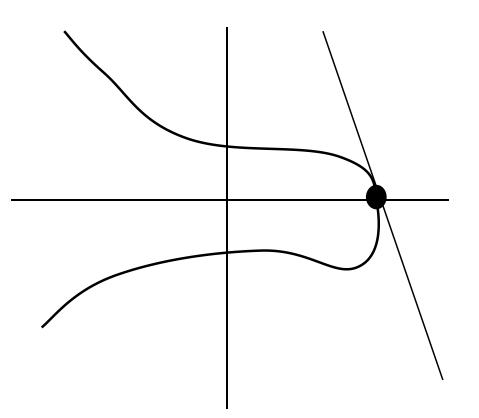
\includegraphics[width=1\linewidth]{img/part4/chapter19/1.png}}
        \end{minipage}
                               &
        \begin{minipage}[b]{0.5\columnwidth}
            \centering
            \raisebox{-1\height}{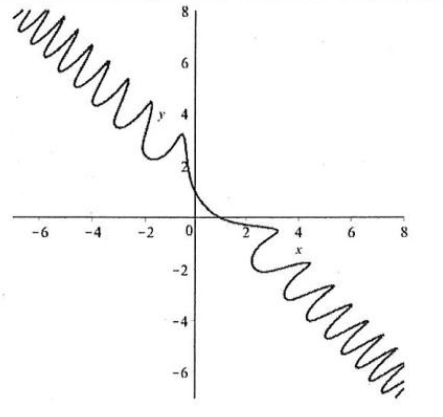
\includegraphics[width=1\linewidth]{img/part4/chapter19/2.png}}
        \end{minipage}
        \\ \hline
    \end{tabular}
\end{table}

For relations like these, there is no way to isolate for either $ x $ or $ y $. Either variable is implicitly defined in the equation in both of the above cases. \\

\begin{exercise}\nonumber
    If $ x^3 + xy + y^2 = 1 $, find $ dy \over dx $ at the point $ (x, y) = (1, 0) $. \\

    \begin{align}
        \\
        \\
        \\
        \\
        \\
        \\
        \\
        \\
    \end{align}
\end{exercise}

\begin{exercise}\nonumber
    If $ sin(tx^3) + ln(t^2 + x) = 0 $, find $ dx \over dt $. \\

    \begin{align}
        \\
        \\
        \\
        \\
        \\
        \\
    \end{align}
\end{exercise}

\begin{exercise}\nonumber
    Show that if $ e^{2xy} +e^x + e^y = y $ that $ {dx \over dy} = {1 \over {dy \over dx}} $. \\

    \begin{align}
        \\
        \\
        \\
        \\
        \\
        \\
        \\
        \\
        \\
        \\
        \\
        \\
        \\
        \\
        \\
        \\
    \end{align}
\end{exercise}

\begin{exercise}\nonumber
    If $ x^3 + x = y $, find $ d^2y \over dx^2 $. \\

    \begin{align}
        \\
        \\
        \\
        \\
        \\
        \\
        \\
        \\
        \\
        \\
        \\
    \end{align}
\end{exercise}

\begin{exercise}\nonumber
    A 10m ladder leans against a perpendicular wall. \\

    (a) The top of the ladder slides down the wall at 0.5m/s. How fast is the foot of the ladder moving at the moment the top of the ladder touches the wall 8m above the ground? \\

    \begin{figure}[H]
        \centering
        \begin{tikzpicture}[scale=0.6]
            \draw[->] (-1,0) -- (6,0);
            \draw[->] (0,-1) -- (0,6);
            \draw[-,very thick,red] (0,0) -- (3,0) node[below] {$ x = 6 $};
            \draw[-,very thick,red] (0,0) -- (0,4) node[left] {$ y = 8 $};
            \draw[-,very thick,red] (0,4) -- (3,0);
        \end{tikzpicture}
    \end{figure}

    KNOWN: $ {dy \over dt} = -0.5, y=8 $

    \begin{align}
        \\
        \\
        \\
        \\
        \\
        \\
        \\
        \\
    \end{align}

    (b) Consider the angle that the ladder makes with the ground. How fast is this angle changing at that exact moment? \\

    WANT: $ d\theta \over dt $

    \begin{align}
        \\
        \\
        \\
        \\
        \\
    \end{align}
\end{exercise}

\chapter{Logarithmic Differentiation}

\section{Logarithmic Differentiation}

Logarithmic differentiation allows us to take the derivatives of more complicated expressions. The derivative rules give us a way to quickly differentiate expression like $x^5$, $e^{4x}$, $ 2^x $. But what about $x^x$? \\

\begin{exercise}\nonumber
    Use a table of values to sketch the function $ f(x) = x^x $. \\

    \begin{figure}[H]
        \centering
        \begin{tabular}{|c|c|c|c|}
            \hline
            $ x > 0 $ & $ f(x) $ & $ x < 0 $ & $ f(x) $ \\
            \hline
                      &          &           &          \\
            \hline
                      &          &           &          \\
            \hline
                      &          &           &          \\
            \hline
                      &          &           &          \\
            \hline
        \end{tabular}
    \end{figure}

    \begin{figure}[H]
        \centering
        \begin{tikzpicture}[scale=0.6, yscale=0.7]
            \draw[->] (-2,0) -- (4,0) node[right] {$ x $};
            \draw[->] (0,-2) -- (0,7) node[above] {$ y $};
        \end{tikzpicture}
        \caption{$ y = x ^ x $ when $ x > 0 $}
    \end{figure}

    \begin{figure}[H]
        \centering
        \begin{tikzpicture}[scale=0.6]
            \draw[->] (-5,0) -- (2,0) node[right] {$ x $};
            \draw[->] (0,-3) -- (0,2) node[above] {$ y $};
        \end{tikzpicture}
        \caption{$ y = x ^ x $ when $ x < 0 $}
    \end{figure}
\end{exercise}

$ x^x $ is indeterminate when $ x = 0 $. Because the domain of $ x^x $ is extremely complicated when $ x < 0 $, this function is often only considered for $ x > 0 $. \\

So, how do we determine the derivative of this function? With logarithmic differentiation, we take the ln() of both side. Then we use log rules to simplify what we get before we finish by differentiating implicitly. \\

\begin{exercise}\nonumber
    If $ y = (cos(\pi x))^{2x} $, find $  dy \over dx $.

    \begin{align}
        \\
        \\
        \\
        \\
        \\
        \\
    \end{align}
\end{exercise}

\begin{exercise}\nonumber
    If $ y = \left(cos(\pi x)\right)^{2x} $, find $  dy \over dx $.

    \begin{align}
        \\
        \\
        \\
        \\
        \\
    \end{align}
\end{exercise}

It would be tedious to differentiate expression like $ y = {(x-2)^2(3x+1)^3\sqrt{x^2+2} \over (x-1)(x+10)^{10}} $ using product and quotient rules, and put pus at a high risk for making mistakes. We can use logarithms to simplify problems. It is technically an important step that we take the absolute value of both sides first that we aren��t considering the $ ln() $ of a negative number. \\

\begin{exercise}\nonumber
    If $ y = {(x-2)^2(3x+1)^3\sqrt{x^2+2} \over (x-1)(x+10)^{10}} $, find $ dy \over dx $. \\

    \begin{align}
        \\
        \\
        \\
        \\
        \\
        \\
        \\
        \\
        \\
        \\
        \\
        \\
    \end{align}
\end{exercise}

\chapter{Differential Approximation}

\section{Differential Approximation}

Differential approximation allows us to calculate estimates if numbers that would be impossible to find by hand. For example, we know what $ sin(\pi) $ is, but what about $ sin(3) $? \\

The idea is simple. Given a function $ f(x) $ and a difficult-to-evaluate value of $ x = a $, we want to follow this process to estimate $  f(a) $: \\

\begin{enumerate}
    \item
          Find a nearby value $ a^* $ at which $ f $ is easy to calculate. \\

    \item
          Find the tangent line there, called $ L(x) $, with slope $ f'(a^*) $. \\

    \item
          Estimate $ f(a) $ by using the height $ L(a) $ instead. \\
\end{enumerate}

\begin{figure}[H]
    \centering
    \begin{tikzpicture}[scale=0.7]
        \draw[->] (-1,0) -- (4,0) node[right] {$ x $};
        \draw[->] (0,-4) -- (0,4) node[above] {$ y $};
        \draw [very thick,color=red,domain=0.1:4,samples=100] plot (\x,{log2(\x)});
        \draw[-,red,very thick] (-1,-4) -- (3,4);
    \end{tikzpicture}
\end{figure}

\begin{exercise}\nonumber
    Estimate $ sin(3) $ using differential approximation. \\

    \vspace{8cm}
\end{exercise}

\begin{exercise}\nonumber
    Estimate $ \sqrt{65} $ using differential approximation.

    \begin{align}
        \\
        \\
        \\
        \\
        \\
        \\
        \\
        \\
        \\
        \\
        \\
        \\
        \\
        \\
        \\
        \\
    \end{align}
\end{exercise}
\part{Antiderivatives}

\chapter{The Indefinite Integral}

\section{The Indefinite Integral}

How do we undo a derivative? If we were given the derivative of a function $ f'(x) $, how could we find the original function $ f(x) $? The answer is called the antiderivative of $ f(x) $, which we will denote by the associated capital letter $ F(x) $. \\

Another way to think about this question is: "What function do I have to take the derivative of in order to get the answer?" The antiderivative of $ f(x) = 2x $ is $ x^2 $. \\

But what about $ F(x) = x^2 + 1 $? This works too! In fact, since when we take the derivative of a constant, we get zero. We could have chosen any constant. As a result, we report our antiderivative in its most general form $ x^2 + C $. The constant $ C $ is an important part of the antiderivative. \\

Notationally, we denote the operation of take the antiderivative (known as integration) as: \\

$$
    \int 2x \ dx = x^2 + C
$$

This is also called the indefinite integral of the function $ f(x) $, or sometimes just the integral of $ f(x) $, where $ f(x) $ is called the integrand. \\

That was a pretty simple example, so how do we find antiderivatives of more complicated expressions? In much the same way as we did with derivatives, we can generate a set of rules for finding antiderivatives, derived simply by thinking of our familiar derivative rules in reverse. \\

\section{Basic Antiderivative Rules}

The power rule for derivatives multiplies by the power and then subtracts one from the power. Reversing these operations means that we add one to the power and divide by the new power. \\

\subsection{Reverse Power Rule}

\begin{theorem}[Reverse Power Rule]
    \begin{align}
        \int x^n \ dx = {x^{n+1} \over n+1} + C,\ where\ n \ne -1
    \end{align}
\end{theorem}

\begin{exercise}\nonumber
    Find the anitiderivatives. \\

    (a)
    \begin{align}
         & \int x^6 \ dx       \\
         & = {x^7 \over 7} + C \\
    \end{align}

    (b)
    \begin{align}
         & \int \sqrt[4]{t} \ dt       \\
         & = \int t^{1 \over 4} \ dt   \\
         & = {t^{5/4} \over {5/4}} + C \\
         & = {4t^{5/4} \over 5} + C    \\
    \end{align}

    (c)
    \begin{align}
         & \int {1 \over x^{5/3}} \ dx  \\
         & = \int x^{-{5 \over 3}} \ dx \\
         & = {x^{-2/3} \over -2/3} + C  \\
         & = -{3 \over 2x^{2/3}} + C
    \end{align}
\end{exercise}

\subsection{Antiderivative of Zero}

\begin{theorem}[Antiderivative of Zero]
    \begin{align}
        \int 0 \ dx = C
    \end{align}
\end{theorem}

\subsection{Antiderivative of a Constant}

\begin{theorem}[Antiderivative of a Constant]
    \begin{align}
        \int k \ dx = kx + C,\ where\ k\ is\ any\ constant
    \end{align}
\end{theorem}

\begin{exercise}\nonumber
    Find the anitiderivatives.

    \begin{align}
         & \int \pi \ dx \\
         & = \pi x + C
    \end{align}
\end{exercise}

\subsection{Multiplicative Constants}

\begin{theorem}[Multiplicative Constantst]
    \begin{align}
        \int kf(x) \ dx = k \int f(x) \ dx
    \end{align}
\end{theorem}

\begin{exercise}\nonumber
    Find the anitiderivatives. \\

    (a)
    \begin{align}
         & \int 4x^7 \ dx                    \\
         & = 4 \int x^7 \ dx                 \\
         & = 4\left({x^8 \over 8} + C\right) \\
         & = {x^8 \over 2} + C               \\
    \end{align}

    (b)
    \begin{align}
         & \int {\pi \over \sqrt{t}} \ dt      \\
         & = \pi \int t^{-{1 \over 2}} \ dt    \\
         & = \pi \cdot {t^{1/2} \over 1/2} + C \\
         & = 2\pi t^{1/2} + C
    \end{align}
\end{exercise}

\subsection{Sum / Difference}

\begin{theorem}[Sum / Difference]
    \begin{align}
        \int (f(x) \pm g(x)) \ dx = \int f(x) \ dx \pm \int g(x) \ dx
    \end{align}
\end{theorem}

\begin{exercise}\nonumber
    Find the anitiderivatives. \\

    (a)
    \begin{align}
         & \int (3x^2 + 5) \ dx      \\
         & = {3x^3 \over 3} + 5x + C \\
         & = x^3 + 5x + C            \\
    \end{align}

    (b)
    \begin{align}
         & \int \left({1 \over x^3} - {2 \over x^2}\right) \ dx      \\
         & = \int (x^{-3} - 2x^{-2}) \ dx                            \\
         & = {x^{-2} \over -2} - 2\left({x^{-1} \over -1}\right) + C \\
         & = -{1 \over 2x^2} + {2 \over x} + C
    \end{align}
\end{exercise}

\subsection{Trigonometric Functions}

\begin{theorem}[Trigonometric Functions]
    \begin{align}
        \int sin(x) \ dx       & = -cos(x) + C \\
        \int cos(x) \ dx       & = sin(x) + C  \\
        \int csc^2(x) \ dx     & = -cot(x) + C \\
        \int sec^2(x) \ dx     & = tan(x) + C  \\
        \int sec(x)tan(x) \ dx & = sec(x) + C  \\
        \int csc(x)cot(x) \ dx & = -csc(x) + C
    \end{align}
\end{theorem}

\subsection{Exponential / Logarithmic}

\begin{theorem}[Exponential / Logarithmic]
    \begin{align}
        \int a^xln(a) \ dx         & = a^x + C      \\
        \int e^xln(e) \ dx         & = e^x + C      \\
        \int {1 \over xln(a)} \ dx & = log_a|x| + C \\
        \int {1 \over x} \ dx      & = ln|x| + C
    \end{align}
\end{theorem}

\begin{exercise}\nonumber
    Find the anitiderivatives. \\

    (a)
    \begin{align}
         & \int 4^xln(4) + 5e^x - {6 \over x} \ dx \\
         & = 4^x + 5e^x - 6ln|x| + C               \\
    \end{align}

    (b)
    \begin{align}
         & \int 3^z \ dz                        \\
         & = {1 \over ln(3)} \int 3^zln(3) \ dz \\
         & = {1 \over ln(3)} \cdot 3^z + C
    \end{align}
\end{exercise}

Sometimes we need to manipulate the integral a little bit before we can apply the rules. \\

\begin{exercise}\nonumber
    Find the anitiderivatives. \\

    (a)
    \begin{align}
         & \int {2s^3 - 5s^4 \over 3s^2} \ ds                                      \\
         & = \int {2 \over 3}s - {5 \over 3}s^2 \ ds                               \\
         & = {2 \over 3} \cdot {s^2 \over 2} - {5 \over 3} \cdot {s^3 \over 3} + C \\
         & = {s^2 \over 3} - {5s^3 \over 9} + C                                    \\
    \end{align}

    (b)
    \begin{align}
         & \int \left({1 \over x} + {1 \over x^2}\right)\left(3 + 2x^2\right) \ dx \\
         & = \int {3 \over x} + 2x + {3 \over x^2} + 2 \ dx                        \\
         & = 3ln|x| + x^2 + 3 \cdot {x^{-1} \over -1} + 2x + C                     \\
         & = 3ln|x| + x^2 + {3 \over x} + 2x + C
    \end{align}
\end{exercise}

\chapter{Chain Rule in Reverse}

\section{Chain Rule in Reverse}

The derivative of $ f(u(x)) $ is $ f'(u(x))u'(x) $, so \\

\begin{theorem}[Chain Rule in Reverse]
    \begin{align}
        \int f'(u(x))u'(x) \ dx = f(u(x)) + C
    \end{align}
\end{theorem}

Notice that in the integration, the $ u'(x) $ piece disappears, being absorbed back into $ f(x) $. The steps for finding the antiderivative of composition functions are as follows: \\

\begin{enumerate}
    \item
          Identify the core layer $ u(x) $.

    \item
          Identify the derivative of the core layer $ u'(x) $.

    \item
          Identify the outer layer $ f' $, and integrate $ f' $ leaving $ u(x) $ inside.
\end{enumerate}

\begin{exercise}\nonumber
    Find the anitiderivatives. \\

    (a)
    \begin{align}
         & \int (6x^2 + 1)sin(2x^3 + x) \ dx \\
        \\
         & u = 2x^3 + x                      \\
         & u' = 6x^2 + 1                     \\
        \\
         & \int (6x^2 + 1)sin(2x^3 + x) \ dx \\
         & = -cos(2x^3 + x) + C              \\
    \end{align}

    (b)
    \begin{align}
         & \int sec^2(4t) \ dt                \\
        \\
         & u = 4t                             \\
         & u' = 4                             \\
        \\
         & \int sec^2(4t) \ dt                \\
         & = {1 \over 4} \int 4sec^2(4t) \ dt \\
         & = {1 \over 4}tan(4t) + C           \\
    \end{align}

    (c)
    \begin{align}
         & \int 4x^3(3x^4 - 1)^{14} \ dx                      \\
        \\
         & u = 3x^4 - 1                                       \\
         & u' = 12x^3                                         \\
        \\
         & \int 4x^3(3x^4 - 1)^{14} \ dx                      \\
         & = {1 \over 3} \int 12x^3(3x^4 - 1)^14 \ dx         \\
         & = {1 \over 3} \cdot {(3x^4 - 1)^{15} \over 15} + C \\
         & = {(3x^4 - 1)^{15} \over 45} + C                   \\
    \end{align}

    (d)
    \begin{align}
         & \int {e^{1 \over x} \over 4x^2} \ dx                 \\
        \\
         & u = {1 \over x}                                      \\
         & u' = -{1 \over x^2}                                  \\
        \\
         & \int {e^{1 \over x} \over 4x^2} \ dx                 \\
         & = {1 \over 4} \int {1 \over x^2}e^{1 \over x} \ dx   \\
         & = -{1 \over 4} \int -{1 \over x^2}e^{1 \over x} \ dx \\
         & = -{1 \over 4}e^{1 \over x} + C
    \end{align}
\end{exercise}

\begin{exercise}\nonumber
    Integrate in one step. \\

    \begin{align}
         & \int e^{-2t} + sin(3t) + cos\left({1 \over 4}t\right) \ dt                     \\
         & = -{1 \over 2}e^{-2t} - {1 \over 3}cos(3t) + 4sin\left({1 \over 4}t\right) + C
    \end{align}
\end{exercise}

\chapter{The Method of Substitution}

\section{The Method of Substitution}

The idea behind the method of substitution is to change a difficult integral in terms of one variable into an easier integral in terms of some other variable using a substitution. \\

\begin{theorem}[The Method of Substitution]
    \begin{align}
        \int f'(u(x)) \ {du \over dx} = \int f'(u) \ du
    \end{align}
\end{theorem}

\begin{exercise}\nonumber
    The method of substitution.

    \begin{align}
        \int (6x + 4)(3x^2 + 4x)^5 \ dx
    \end{align}

    \begin{enumerate}
        \item
              Identify the core layer $ u(x) = 3x^2 +4x $. \\

        \item
              Find the derivative of the core $ {du \over dx} = 6x + 4 $. \\

        \item
              Transform from an integral in $ x $ to an integral in the new variable $ u $ using the change of variable theorem. \\
              \begin{align}
                   & \int (6x + 4)(3x^2 + 4x)^5 \ dx \\
                   & = \int {du \over dx}u^5 \ dx    \\
                   & = \int u^5 \ du                 \\
                   & = {u^6 \over 6} + C
              \end{align}

        \item
              Convert back to the original variable by substituting $ u(x) $ back in.
              \begin{align}
                   & {u^6 \over 6} + C             \\
                   & = {(3x^2 + 4x)^6 \over 6} + C
              \end{align}
    \end{enumerate}
\end{exercise}

\begin{exercise}\nonumber
    Calculate using the method of substitution. \\

    (a)
    \begin{align}
                                         & \int sin(x)e^{5cos(x)} \ dx                     \\
        \\
        u                                & = 5cos(x)                                       \\
        {du \over dx}                    & = -5sin(x)                                      \\
        -{1 \over 5} \cdot {du \over dx} & = sin(x)                                        \\
        \\
                                         & \int sin(x)e^{5cos(x)} \ dx                     \\
                                         & = \int -{1 \over 5} \cdot {du \over dx}e^u \ dx \\
                                         & = \int -{1 \over 5}e^u \ du                     \\
                                         & = -{1 \over 5}e^u + C                           \\
                                         & = -{1 \over 5}e^{5cos(x)} + C                   \\
    \end{align}

    (b)
    \begin{align}
                                        & \int {x \over (5x + 7)^3} \ dx                                                        \\
        \\
        u                               & = 5x + 7 \rightarrow x = {1 \over 5}{u - 7}                                           \\
        {du \over dx}                   & = 5                                                                                   \\
        {1 \over 5} \cdot {du \over dx} & = 1                                                                                   \\
        \\
                                        & \int {x \over (5x + 7)^3} \ dx                                                        \\
                                        & = \int {x \cdot 1 \over (5x+7)^3} \ dx                                                \\
                                        & = \int{{1 \over 5}(u - 7) \over u^3}\left({1 \over 5} \cdot {du \over dx}\right) \ dx \\
                                        & = {1 \over 25} \int {u - 7 \over u^3} \ du                                            \\
                                        & = {1 \over 25} \int u^{-2} - 7u^{-3} \ du                                             \\
                                        & = {1 \over 25}\left({u^{-1} \over -1} - {{7u^{-2} \over -2}}\right) + C               \\
                                        & = -{1 \over 25} \cdot {1 \over 5x+7} + {7 \over 50} \cdot {1 \over (5x+7)^2} + C      \\
    \end{align}

    (c)
    \begin{align}
           & \int xsec(3x^2)tan(3x^2) \ dx                \\
        \\
        u  & = 3x^2                                       \\
        u' & = 6x                                         \\
        \\
           & \int xsec(3x^2)tan(3x^2) \ dx                \\
           & = {1 \over 6} \int 6xsec(3x^2)tan(3x^2) \ dx \\
           & = {1 \over 6}sec(3x^2) + C                   \\
    \end{align}

    (d)
    \begin{align}
           & \int {-{1 \over t^2} + 1 \over \sqrt{{1 \over t} + t}} \ dt                            \\
        \\
        u  & = {1 \over t} + t                                                                      \\
        u' & = -{1 \over t^2} + 1                                                                   \\
        \\
           & \int {-{1 \over t^2} + 1 \over \sqrt{{1 \over t} + t}} \ dt                            \\
           & = \int \left(-{1 \over t^2} + 1\right)\left({1 \over t} + t\right)^{-{1 \over 2}} \ dt \\
           & = {\left({1 \over t} +t\right)^{1/2} \over 1/2} + C                                    \\
           & = 2\left({1 \over t} + t\right)^{1/2} + C                                              \\
    \end{align}

    (e)
    \begin{align}
           & \int (1 + 900x)^{1/15000} \ dx                                       \\
        \\
        u  & = 1 + 900x                                                           \\
        u' & = 900                                                                \\
        \\
           & \int (1 + 900x)^{1/15000} \ dx                                       \\
           & = {1 \over 900} \int 900(1 + 900x)^{1/15000} \ dx                    \\
           & = {1 \over 900} \cdot {(1+900x)^{15001/15000} \over 15001/15000} + C \\
    \end{align}

    (f)
    \begin{align}
         & \int sin(\theta)(cos^3\theta - cos^5\theta) \ d\theta                \\
         & = \int sin(\theta)cos(\theta)^3 - sin(\theta)cos(\theta)^5 \ d\theta \\
         & = -{cos^4\theta \over 4} + {cos^6\theta \over 6} + C                 \\
    \end{align}

    (g)
    \begin{align}
           & \int {7x \over 4x^2 + 9} \ dx                     \\
        \\
        u  & = 4x^2 + 9                                        \\
        u' & = 8x                                              \\
        \\
           & \star \int {u'(x) \over u(x)} \ dx = ln|u(x)| + C \\
        \\
           & \int {7x \over 4x^2 + 9} \ dx                     \\
           & = {7 \over 8} \int {8x \over 4x^2 + 9} \ dx       \\
           & = {7 \over 8} \cdot ln|4x^2 + 9| + C              \\
           & = {7 \over 8} \cdot kn(4x^2 + 9) + C              \\
    \end{align}

    (h)
    \begin{align}
                                        & \int (2x + 5) \cdot \sqrt[3]{3x + 1} \ dx                                                    \\
        \\
        u                               & = 3x + 1                                                                                     \\
        {1 \over 3}(u - 1)              & = 1                                                                                          \\
        {1 \over 3}u - {1 \over 3}      & = x                                                                                          \\
        {2 \over 3}u - {2 \over 3}      & = 2x                                                                                         \\
        {2 \over 3}u - {2 \over 3} + 5  & = 2x + 5                                                                                     \\
        {2 \over 3}u + {13 \over 3}     & = 2x + 5                                                                                     \\
        {1 \over 3}(2u + 13)            & = 2x + 5                                                                                     \\
        \\
        u                               & = 3x + 1                                                                                     \\
        {du \over dx}                   & = 3                                                                                          \\
        {1 \over 3} \cdot {du \over dx} & = 1                                                                                          \\
        \\
                                        & \int (2x + 5) \cdot \sqrt[3]{3x + 1} \ dx                                                    \\
                                        & = \int {1 \over 3}(2u + 13) \sqrt[3]{u} {1 \over 3} \cdot {du \over dx}                      \\
                                        & = {1 \over 9} \int (2u + 13) u^{1/3} \ du                                                    \\
                                        & = {1 \over 9}\left(2 \cdot {u^{7/3} \over {7/3}} + 13 \cdot {u^{4/3} \over {4/3}}\right) + C \\
                                        & = {2 \over 21}(3x + 1)^{7/3} + {13 \over 12}(3x + 1)^{4/3} + C
    \end{align}
\end{exercise}

\chapter{Definite Integrals}

\section{Riemann Sum}

Suppose we wanted to find the area underneath the graph of a straight line that lies above the x-axis, between $ x = a $ and $  x = b $. Since we have formulas for finding the area of basic shapes, we can easily figure this out. \\

\begin{figure}[H]
    \centering
    \begin{tikzpicture}
        \fill[yellow](1,0) -- (1,2) -- (3.5,4.5) to[out=45,in=35] (4,4.8) -- (4,0) -- cycle;
        \draw[thick,-latex] (-2,0) -- (6,0);
        \draw[thick,-latex] (0,-1) -- (0,6);
        \draw[very thick,black] (-0.8,0.2) -- (3.5,4.5) to[out=45,in=135] node[pos=0.5,above,font=\large]{$ f(x) $} (5,4.5);
        \draw[very thick,dashed,gray]
        (1,0) node[below,black] {$a$} -- (1,2)
        (4,0) node[below,black] {$b$} -- (4,4.8);
    \end{tikzpicture}
\end{figure}

But what about finding the area underneath the graph of a general curve $ y = f(x) $ and above the x-axis between $  x = a $ and $ x = b $? \\

Bernhard Riemann's idea was to carve up the desired area into rectangle and user their area to estimate the true area. He called this the Riemann Sum and it goes as follows: \\

\begin{enumerate}
    \item
          Create a partition $ P $, dividing up the interval $ [a, b] $ into n subintervals $ I_1, I_2, \dots, I_n $. \\

    \item
          Choose an x-value (called it $ x_k $) in each subinterval $ I_k $. \\

    \item
          For each $ x_k $ we choose, draw a rectangle with height $ f(x_k) $ and a width spanning $ I_k $ ($ \Delta x_k $). \\
\end{enumerate}

\begin{figure}[H]
    \centering
    \begin{tikzpicture}[scale=1.2]
        \def\a{1.7}
        \def\b{5.7}
        \def\c{3.7}
        \def\L{0.5} % width of interval

        \pgfmathsetmacro{\Va}{2*sin(\a r+1)+4} \pgfmathresult
        \pgfmathsetmacro{\Vb}{2*sin(\b r+1)+4} \pgfmathresult
        \pgfmathsetmacro{\Vc}{2*sin(\c r+1)+4} \pgfmathresult

        \draw[->,very thick] (-0.5,0) -- (7,0) coordinate (x axis) node[below] {$x$};
        \draw[->,very thick] (0,-0.5) -- (0,7) coordinate (y axis) node[left] {$y$};
        \foreach \f in {1.7,2.2,...,6.2} {\pgfmathparse{2*sin(\f r+1)+4} \pgfmathresult
                \draw[fill=blue!20] (\f-\L/2,\pgfmathresult |- x axis) -- (\f-\L/2,\pgfmathresult) -- (\f+\L/2,\pgfmathresult) -- (\f+\L/2,\pgfmathresult |- x axis) -- cycle;}
        \node at (\a-\L/2,-5pt) {\footnotesize{$a$}};
        \node at (\b+\L/2+\L,-5pt) {\footnotesize{$b$}};
        \draw[blue,very thick,smooth,samples=100,domain=1.45:6.2] plot(\x,{2*sin(\x r+1)+4});
    \end{tikzpicture}
\end{figure}

The area of rectangle $ k $ is:
$$
    f(x_k) \cdot \Delta x_k
$$

The total area of all the rectangles is:
$$
    f(x_1) \cdot \Delta x_1 + f(x_2) \cdot \Delta x_2 + \dots + f(x_n) \cdot \Delta x_n = \sum_{k=1}^{n} f(x_k) \cdot \Delta x_k
$$

\begin{exercise}\nonumber
    Use the Riemann Sum to estimate the area below $ y = sin({1 \over 2}x) $ and above the x-axis, between $ x = 0 $ and $ x = 2\pi $. Use a partition of 4 subintervals. \\

    \begin{figure}[H]
        \centering
        \begin{tikzpicture}[
                declare function={
                        f(\x)=sin(deg(0.5*\x));
                    },
                xscale=0.5
            ]
            \begin{axis}[
                    axis lines = middle,
                    xtick ={1,4},
                    ytick ={0},
                    xticklabels = {$a$,$b$},
                    ymin = -0.2,
                    ymax = 2,
                    xmin = -0.2,
                    xmax = 7,
                    x=2cm,y=2cm,
                    axis line style = thick,
                ]

                \addplot [
                    domain=0:6.3,
                    samples=300,
                    line width=1pt,
                    fill=red, draw=none,
                    fill opacity=0.2
                ] {f(x)} \closedcycle;

                \addplot [
                    domain=0:6.3,
                    samples=300,
                    line width = 1pt, red
                ] {f(x)};

                \addplot [
                    ycomb, thick, red,
                    no markers,
                    samples at={1,3,5}
                ] {f(x)};
            \end{axis}
            \draw[dashed,red] (2.4, 1.3) -- (0.3, 1.3);
            \draw[dashed,red] (6.1, 2.4) -- (2.4, 2.4) -- (2.4, 0);
            \draw[dashed,red] (10.2, 1.55) -- (6.4, 1.55);
            \draw[dashed,red] (12.9, 0.4) -- (10.4, 0.4);
        \end{tikzpicture}
    \end{figure}

    \begin{align}
             & \Delta x_k = {2 \pi \over 4} = {\pi \over 2}                                                                                                                                                                                                                             \\
        \\
        Area & = \left({\pi \over 2}\right)\left(sin\left({1 \over 2} \cdot {{\pi \over 2}}\right)\right) + \left({\pi \over 2}\right)\left(sin\left({1 \over 2} \cdot \pi\right)\right) + \left({\pi \over 2}\right)\left(sin\left({1 \over 2} \cdot {3 \pi \over 2}\right)\right) + 0 \\
             & = {\pi \over 2}\left({1 \over \sqrt{2}} + 1 + {1 \over \sqrt{2}}\right)                                                                                                                                                                                                  \\
             & = {1 \over 2}\left({2 \over \sqrt{2}} + 1\right) \ unit^2
    \end{align}
\end{exercise}

So, what happens as make the rectangles skinnier? \\

\begin{figure}[H]
    \centering
    \begin{tikzpicture}[scale=0.6,
            declare function={
                    f(\x)=2+sin(deg(\x-2))+sin(deg(3*\x))/2+sin(deg(5*\x))/8 + sin(deg(7*\x))/28;
                }
        ]
        \begin{axis}[
                axis lines = middle,
                xtick ={1,4},
                ytick ={0},
                xticklabels = {$a$,$b$},
                ymin = -0.2,
                ymax = 3.7,
                xmin = -0.2,
                xmax = 5.2,
                x=2cm,y=2cm,
                axis line style = thick,
            ]

            \addplot [
                domain=1:4,
                samples=300,
                line width=1pt,
                fill=red, draw=none,
                fill opacity=0.2
            ] {f(x)} \closedcycle;

            \addplot [
                domain=0:5,
                samples=300,
                line width = 1pt, red
            ] {f(x)};

            \addplot [
                ycomb, thick, red,
                no markers,
                samples at={1,2,...,4}
            ] {f(x)};
        \end{axis}
    \end{tikzpicture}
\end{figure}

\begin{figure}[H]
    \centering
    \begin{tikzpicture}[scale=0.6,
            declare function={
                    f(\x)=2+sin(deg(\x-2))+sin(deg(3*\x))/2+sin(deg(5*\x))/8 + sin(deg(7*\x))/28;
                }
        ]
        \begin{axis}[
                axis lines = middle,
                xtick ={1,4},
                ytick ={0},
                xticklabels = {$a$,$b$},
                ymin = -0.2,
                ymax = 3.7,
                xmin = -0.2,
                xmax = 5.2,
                x=2cm,y=2cm,
                axis line style = thick,
            ]

            \addplot [
                domain=1:4,
                samples=300,
                line width=1pt,
                fill=red, draw=none,
                fill opacity=0.2
            ] {f(x)} \closedcycle;

            \addplot [
                domain=0:5,
                samples=300,
                line width = 1pt, red
            ] {f(x)};

            \addplot [
                ycomb, thick, red,
                no markers,
                samples at={1,1.5,...,4}
            ] {f(x)};
        \end{axis}
    \end{tikzpicture}
\end{figure}

\begin{figure}[H]
    \centering
    \begin{tikzpicture}[scale=0.6,
            declare function={
                    f(\x)=2+sin(deg(\x-2))+sin(deg(3*\x))/2+sin(deg(5*\x))/8 + sin(deg(7*\x))/28;
                }
        ]
        \begin{axis}[
                axis lines = middle,
                xtick ={1,4},
                ytick ={0},
                xticklabels = {$a$,$b$},
                ymin = -0.2,
                ymax = 3.7,
                xmin = -0.2,
                xmax = 5.2,
                x=2cm,y=2cm,
                axis line style = thick,
            ]

            \addplot [
                domain=1:4,
                samples=300,
                line width=1pt,
                fill=red, draw=none,
                fill opacity=0.2
            ] {f(x)} \closedcycle;

            \addplot [
                domain=0:5,
                samples=300,
                line width = 1pt, red
            ] {f(x)};

            \addplot [
                ycomb, thick, red,
                no markers,
                samples at={1,1.1,...,4}
            ] {f(x)};
        \end{axis}
    \end{tikzpicture}
\end{figure}

As the width of the rectangles decreases, the accuracy of the estimate increases. So, what happens if we let the width of all the rectangles in the partition approach 0? \\

Notationally:

$$
    \lim\limits_{\substack{n \rightarrow \infty \\ \left\|p\right\| \rightarrow 0}} \sum_{k=1}^{n} f(x_k) \cdot \Delta x_k
$$

We should get the exact area, that is, our estimate is no longer just an estimate. \\

Notationally, instead of limit, we write it as: \\

\begin{theorem}[Definite Integral]
    \begin{align}
        \int_{x = a}^{b} f(x) \ dx
    \end{align}
\end{theorem}

\section{Definite Integral}

For all of the following, suppose that $ k $, $ a $, $ b $, and $ c $ are constants with $ a < b < c $, and that $ f $ and $ g $ are integrable functions on the domain of integration. \\

\begin{theorem}[Definite Integral]
    \begin{align}
        \int_a^b k \ dx = (b - a)k
    \end{align}
\end{theorem}

\begin{figure}[H]
    \centering
    \begin{tikzpicture}[scale=0.6,
            declare function={
                    f(\x)=2;
                }
        ]
        \begin{axis}[
                axis lines = middle,
                xtick ={1,4},
                ytick ={0},
                xticklabels = {$a$,$b$},
                ymin = -0.2,
                ymax = 3.7,
                xmin = -0.2,
                xmax = 5.2,
                x=2cm,y=2cm,
                axis line style = thick,
            ]

            \addplot [
                domain=1:4,
                samples=300,
                line width=1pt,
                fill=red, draw=none,
                fill opacity=0.2
            ] {f(x)} \closedcycle;

            \addplot [
                domain=0:5,
                samples=300,
                line width = 1pt, red
            ] {f(x)};

            \addplot [
                ycomb, thick, red,
                no markers,
                samples at={1,4}
            ] {f(x)};
        \end{axis}
    \end{tikzpicture}
\end{figure}

\begin{theorem}[Definite Integral]
    \begin{align}
        \int_a^a f(x) \ dx = 0
    \end{align}
\end{theorem}

\begin{figure}[H]
    \centering
    \begin{tikzpicture}[scale=0.6,
            declare function={
                    f(\x)=0.5 * sin(deg(\x)) + 2;
                }
        ]
        \begin{axis}[
                axis lines = middle,
                xtick ={1},
                ytick ={0},
                xticklabels = {$a$},
                ymin = -0.2,
                ymax = 3.7,
                xmin = -0.2,
                xmax = 5.2,
                x=2cm,y=2cm,
                axis line style = thick,
            ]

            \addplot [
                domain=0:5,
                samples=300,
                line width = 1pt, red
            ] {f(x)};

            \addplot [
                ycomb, thick, red,
                no markers,
                samples at={1}
            ] {f(x)};
        \end{axis}
    \end{tikzpicture}
\end{figure}

\begin{theorem}[Definite Integral]
    \begin{align}
        \int_b^a f(x) \ dx = -\int_a^b f(x) \ dx
    \end{align}
\end{theorem}

\begin{figure}[H]
    \centering
    \begin{tikzpicture}[scale=0.6,
            declare function={
                    f(\x)=0.5 * sin(deg(\x)) + 2;
                }
        ]
        \begin{axis}[
                axis lines = middle,
                xtick ={1,4},
                ytick ={0},
                xticklabels = {$a$,$b$},
                ymin = -0.2,
                ymax = 3.7,
                xmin = -0.2,
                xmax = 5.2,
                x=2cm,y=2cm,
                axis line style = thick,
            ]

            \addplot [
                domain=1:4,
                samples=300,
                line width=1pt,
                fill=red, draw=none,
                fill opacity=0.2
            ] {f(x)} \closedcycle;

            \addplot [
                domain=0:5,
                samples=300,
                line width = 1pt, red
            ] {f(x)};

            \addplot [
                ycomb, thick, red,
                no markers,
                samples at={1,4}
            ] {f(x)};
        \end{axis}
    \end{tikzpicture}
\end{figure}

\begin{theorem}[Definite Integral]
    \begin{align}
        \int_a^c f(x) \ dx = \int_a^b f(x) \ dx + \int_b^c f(x) \ dx
    \end{align}
\end{theorem}

\begin{figure}[H]
    \centering
    \begin{tikzpicture}[scale=0.6,
            declare function={
                    f(\x)=0.5 * sin(deg(\x)) + 2;
                }
        ]
        \begin{axis}[
                axis lines = middle,
                xtick ={1,2,4},
                ytick ={0},
                xticklabels = {$a$,$b$,$c$},
                ymin = -0.2,
                ymax = 3.7,
                xmin = -0.2,
                xmax = 5.2,
                x=2cm,y=2cm,
                axis line style = thick,
            ]

            \addplot [
                domain=1:2,
                samples=300,
                line width=1pt,
                fill=red, draw=none,
                fill opacity=0.2
            ] {f(x)} \closedcycle;

            \addplot [
                domain=2:4,
                samples=300,
                line width=1pt,
                fill=blue, draw=none,
                fill opacity=0.2
            ] {f(x)} \closedcycle;

            \addplot [
                domain=0:5,
                samples=300,
                line width = 1pt, red
            ] {f(x)};

            \addplot [
                ycomb, thick, red,
                no markers,
                samples at={1,2,4}
            ] {f(x)};
        \end{axis}
    \end{tikzpicture}
\end{figure}

\begin{theorem}[Definite Integral]
    \begin{align}
        \int_a^b kf(x) \ dx = k \int_a^b f(x) \ dx
    \end{align}
\end{theorem}

\begin{figure}[H]
    \centering
    \begin{tikzpicture}[scale=0.6,
            declare function={
                    f(\x)=0.5 * sin(deg(\x)) + 2;
                    g(\x)=0.5 * sin(deg(\x)) + 1;
                }
        ]
        \begin{axis}[
                axis lines = middle,
                xtick ={1,4},
                ytick ={0},
                xticklabels = {$a$,$b$},
                ymin = -0.2,
                ymax = 3.7,
                xmin = -0.2,
                xmax = 5.2,
                x=2cm,y=2cm,
                axis line style = thick,
            ]

            \addplot [
                domain=0:5,
                samples=300,
                line width = 1pt, red
            ] {f(x)};

            \addplot [
                domain=0:5,
                samples=300,
                line width = 1pt, red
            ] {g(x)};
        \end{axis}
    \end{tikzpicture}
\end{figure}

\begin{theorem}[Definite Integral]
    \begin{align}
        \int_a^b (f(x) \pm g(x))  \ dx = \int_a^b f(x) \ dx \pm \int_a^b g(x) \ dx
    \end{align}
\end{theorem}

\begin{figure}[H]
    \centering
    \begin{tikzpicture}[scale=0.6,
            declare function={
                    f(\x)=0.5 * sin(deg(\x)) + 1;
                    g(\x)=2;
                    h(\x)=0.5 * sin(deg(\x)) + 3;
                }
        ]
        \begin{axis}[
                axis lines = middle,
                xtick ={1,4},
                ytick ={0},
                xticklabels = {$a$,$b$},
                ymin = -0.2,
                ymax = 3.7,
                xmin = -0.2,
                xmax = 5.2,
                x=2cm,y=2cm,
                axis line style = thick,
            ]

            \addplot [
                domain=0:5,
                samples=300,
                line width = 1pt, red
            ] {f(x)};

            \addplot [
                domain=0:5,
                samples=300,
                line width = 1pt, red
            ] {g(x)};
            \addplot [
                domain=0:5,
                samples=300,
                line width = 1pt, red
            ] {h(x)};
        \end{axis}
    \end{tikzpicture}
\end{figure}

\begin{exercise}\nonumber
    Evaluate. \\

    (a)
    \begin{align}
         & \int_1^2 {1 \over t} \ dt        \\
         & = \left[ ln|t| \right|_{t=1}^{2} \\
         & = ln(2) - ln(1)                  \\
         & = ln(2)                          \\
    \end{align}

    (b)
    \begin{align}
         & \int_{-2}^1 x^3 \ dx                  \\
         & = \left. {x^4 \over 4} \right|_{-2}^1 \\
         & = {1^4 \over 4} - {(-2)^4 \over 4}    \\
         & = {1 \over 4} - {16 \over 4}          \\
         & = -{15 \over 4}                       \\
    \end{align}

    (c)
    \begin{align}
         & \int_1^5 s(s^2 + 1) \ ds                                                                  \\
         & = \int_1^5 s^3 + s \ ds                                                                   \\
         & = \left[ {s^4 \over 4} + {s^2 \over 2} \right|_1^5                                        \\
         & = \left({5^2 \over 4} + {5^2 \over 2}\right) - \left({1^2 \over 4} + {1^2 \over 2}\right) \\
         & = {625 \over 4} + {25 \over 2} - {1 \over 4} - {1 \over 2}                                \\
         & = 168                                                                                     \\
    \end{align}

    (d)
    \begin{align}
        \int_{\sqrt{ln(2)}}^{\sqrt{ln(4)}} xe^{x^2} \ dx                        \\
        \\
        u  & = x^2                                                              \\
        u' & = 2x                                                               \\
        \\
           & \int_{\sqrt{ln(2)}}^{\sqrt{ln(4)}} xe^{x^2} \ dx                   \\
           & = {1 \over 2} \int_{\sqrt{ln(2)}}^{\sqrt{ln(4)}} 2xe^{x^2} \ dx    \\
           & = \left[ {1 \over 2} e^{x^2} \right|_{\sqrt{ln(2)}}^{\sqrt{ln(4)}} \\
           & = {1 \over 2}e^{ln(4)} - {1 \over 2}e^{ln(2)}                      \\
           & = {1 \over 2} \cdot 4 - {1 \over 2} \cdot 2                        \\
           & = 2 - 1                                                            \\
           & = 1                                                                \\
    \end{align}

    (e)
    \begin{align}
         & \int_x^{x^2} sin(t) \ dt         \\
         & = \left[ -cos(t) \right|_x^{x^2} \\
         & = -cos(x^2) - (-cos(x))          \\
         & = -cos(x^2) + cos(x)             \\
    \end{align}

    (f)
    \begin{align}
        \int_5^{13} (x + 1)\sqrt{2x - 1} \ dx                                                                                                                                                \\
        \\
        u                               & = 2x - 1                                                                                                                                           \\
        u + 1                           & = 2x                                                                                                                                               \\
        {u \over 2} + {1 \over 2}       & = x                                                                                                                                                \\
        {1 \over 2}u + {3 \over 2}      & = x + 1                                                                                                                                            \\
        {1 \over 2}(u + 3)              & = x + 1                                                                                                                                            \\
        \\
        u                               & = 2x - 1                                                                                                                                           \\
        {du \over dx}                   & = 2                                                                                                                                                \\
        {1 \over 2} \cdot {du \over dx} & = 1                                                                                                                                                \\
        \\
                                        & \int_5^{13} (x + 1)\sqrt{2x - 1} \ dx                                                                                                              \\
                                        & = \int_5^{13} {1 \over 2}(u + 3)\sqrt{u} \cdot {1 \over 2} \cdot {du \over dx} \ dx                                                                \\
                                        & = {1 \over 4} \int_5^{13} (u + 3)u^{1/2} \ du                                                                                                      \\
                                        & = {1 \over 4} \int_5^{13} u^{3/2} + 3u^{1/2} \ du                                                                                                  \\
                                        & = {1 \over 4} \left[ {(2x-1)^{5/2} \over {5/2}} + {3(2x-1)^{3/2} \over {3/2}} \right|_5^{13}                                                       \\
                                        & = {1 \over 4} \left[ {{{25^{5/2}} \over {5/2}} + 3 \cdot {{25^{3/2}} \over {3/2}} - {9^{5/2} \over {5/2}} - 3 \cdot {9^{3/2} \over {3/2}}} \right] \\
                                        & = 10 \cdot 3125 + {1 \over 2} \cdot 125 - {1 \over 10} \cdot 243 - {27 \over 2}                                                                    \\
                                        & = {1686 \over 5}
    \end{align}
\end{exercise}

\chapter{Area Under a Curve}

\section{Area Under a Curve}

\begin{exercise}\nonumber
    Find the area below the curve $ f(x) = sin(x) $ and above the x-axis between $ x = {\pi \over 2} $ and $ x = \pi $. \\

    \begin{figure}[H]
        \centering
        \begin{tikzpicture}[scale=0.8,yscale=0.2]
            \draw[->] (-1,0) -- (8,0) node[right] {$ x $};
            \draw[->] (0,-10) -- (0,30) node[above] {$ y $};
            \draw[very thick,color=red,domain=-1:7] plot (\x,{-2 * (\x - 3.14) ^ 2 + 20});
            \draw[-,very thick,red] (3.14, 0) -- (3.14,20);
            \node at (1.5,-2) [] {$ \pi \over 4 $};
            \node at (3.14,-2) [] {$ \pi \over 2 $};
            \node at (4.8,-2) [] {$ 3\pi \over 4 $};
            \node at (6,-2) [] {$ \pi $};
        \end{tikzpicture}
    \end{figure}

    \begin{align}
        Area & = \int_{x={\pi / 2}}^\pi sin(x) \ dx                        \\
             & = - \left[ cos(x) \right|_{\pi / 2}^\pi                     \\
             & = - \left[ cos(\pi) - cos\left({\pi \over 2}\right) \right] \\
             & = -[-1 - 0]                                                 \\
             & = 1
    \end{align}
\end{exercise}

What if we have a more interesting situation where many curves are involved? For instance, how do we find the area between two curves $ f $ and $ g $? \\

\begin{figure}[H]
    \centering
    \begin{tikzpicture}
        \begin{axis}[
                xlabel={$x$},
                ylabel={$y$},
                xtick={-3,0,1},
                ytick={2},
                samples=100,
                domain=-4:1,
                xmin=-4,xmax=2,
                ymin=-1,ymax=3,
            ]
            \addplot[name path=func, red, very thick, mark=none, ] {sqrt(-x+1)};
            \addplot[name path=line, red, very thick] {2};
            \addplot fill between[
                    of = func and line,
                    soft clip={domain=-3:0},
                    every even segment/.style  = {gray,opacity=.4}
                ];
            \draw[thick,dashed,brown] (axis cs:-3,0) -- (axis cs:-3,2);
        \end{axis}
    \end{tikzpicture}
\end{figure}

$$
\text{Area under Upper} - \text{Area under Lower} = \text{Area expected}
$$

\begin{exercise}\nonumber
    Calculate the area bounded by $ y = 2x + 1 $ and $ y = x^2 - 2x - 3 $. \\

    \begin{figure}[H]
        \centering
        \begin{tikzpicture}[scale=0.8,yscale=0.4]
            \draw[->] (-2,0) -- (7,0) node[right] {$ x $};
            \draw[->] (0,-5) -- (0,15) node[above] {$ y $};
            \draw[very thick,color=red,domain=-2:6] plot (\x,{2 * (\x) + 1});
            \draw[very thick,color=red,domain=-2:5] plot (\x,{(\x) ^ 2 - 2 * \x - 3});
        \end{tikzpicture}
    \end{figure}

    \begin{align}
        2x + 1         & = x^2 - 2x - 3                                                                             \\
        x^2 - 4x - 5   & = 0                                                                                        \\
        (x - 5)(x + 1) & = 0                                                                                        \\
        \begin{cases}
            x_1 & = 5  \\
            x_2 & = -1 \\
        \end{cases}
        \\
        \\
        \text{Area}    & = \text{Upper} - \text{Lower}                                                              \\
                       & = \int_{-1}^5 (2x + 1) - (x^2 - 2x - 3) \ dx                                               \\
                       & = \int_{-1}^5 -x^2 + 4x + 5 \ dx                                                           \\
                       & = \left[ -{x^3 \over 3} + 4 \cdot {x^2 \over 2} + 5x \right|_{-1}^5                        \\
                       & = -{5^3 \over 3} + 2 \cdot 5^2 + 5 \cdot 5 - \left({1 \over 3} + 2 - 5\right)              \\
                       & = -{125 \over 3} + {150 \over 3} + {75 \over 3} - {1 \over 3} - {6 \over 3} + {15 \over 3} \\
                       & = 36
    \end{align}
\end{exercise}

\begin{exercise}\nonumber
    Calculate the area bounded by $ y = -x $, $ y = \sqrt{x} $, and $ y = -x^2 + 2 $ between $ x = 0 $ and $ x = 2 $. \\

    \begin{figure}[H]
        \centering
        \begin{tikzpicture}[scale=0.8]
            \draw[->] (-2,0) -- (5,0) node[right] {$ x $};
            \draw[->] (0,-4) -- (0,4) node[above] {$ y $};
            \draw[very thick,color=red,domain=-2:4] plot (\x,{-(\x)});
            \draw[very thick,color=red,domain=0:5,samples=300] plot (\x,{\x ^ (1/2)});
            \draw[very thick,color=red,domain=-2:2.3] plot (\x,{-(\x) ^ 2 + 2});
            \draw[dashed, very thick,color=blue] (1, 1) -- (1, -1);
            \node at (0.6, 0.2) [blue] {$ A_1 $};
            \node at (1.3, -0.5) [blue] {$ A_2 $};
        \end{tikzpicture}
    \end{figure}

    \begin{align}
        \text{Total Area} & = A_1 + A_2                                                                                                                                      \\
                          & = \int_0^1 \sqrt{x} - (-x) \ dx + \int_1^2 (-x^2 + 2) - (-x) \ dx                                                                                \\
                          & = \int_0^1 x^{1/2} + x \ dx + \int_1^2 -x^2 + x + 2 \ dx                                                                                         \\
                          & = \left[ {{x^{3/2}} \over {3/2}} + {x^2 \over 2} \right|_0^1 + \left[ -{{x^3} \over 3} + {x^2 \over 2} + 2x \right|_1^2                          \\
                          & = \left({1 \over 3/2} + {1 \over 2}\right) - (0 + 0) + \left(-{8 \over 3} + {4 \over 2} + 4\right) - \left(-{1 \over 3} + {1 \over 2} + 2\right) \\
                          & = {2 \over 3} + {1 \over 2} - {8 \over 3} + 2 + 4 + {1 \over 3} - {1 \over 2} - 2                                                                \\
                          & = {7 \over 3}
    \end{align}
\end{exercise}

\begin{exercise}\nonumber
    Find the area bounded by $ y^2 = x + 4 $ and $ y = {1 \over 2}x + {1 \over 2} $. \\

    \begin{figure}[H]
        \centering
        \begin{tikzpicture}[scale=0.8]
            \draw[->] (-5,0) -- (6,0) node[right] {$ x $};
            \draw[->] (0,-3) -- (0,3) node[above] {$ y $};
            \draw[very thick,color=red,domain=-4:6] plot (\x,{0.5 * \x + 0.5});
            \draw[very thick,color=red,domain=-4:6,samples=300] plot (\x,{(\x + 4) ^ (1/2)});
            \draw[very thick,color=red,domain=-4:6,samples=300] plot (\x,{-(\x + 4) ^ (1/2)});
            \draw[dashed,blue] (-3,1) -- (0,1) -- (0,0.5) -- (-3,0.5) -- (-3,1);
        \end{tikzpicture}
    \end{figure}

    \begin{align}
        y^2 = x + 4                    & \rightarrow x = y^2 - 4                                        \\
        y = {1 \over 2}x + {1 \over 2} & \rightarrow x = 2y - 1                                         \\
        \\
        y^2 - 4                        & = 2y - 1                                                       \\
        y^2 - 2y - 3                   & = 0                                                            \\
        (y - 3)(y + 1)                 & = 0                                                            \\
        \begin{cases}
            y_1 & = 3  \\
            y_2 & = -1 \\
        \end{cases}
        \\
        \\
        \text{Area}                    & = \int_{y=-1}^3 (2y - 1) - (y^2 - 4) \ dy                      \\
                                       & = \int_{y=-1}^3 -y^2 + 2y + 3 \ dy                             \\
                                       & = \left[ {-{y^3 \over 3} + {2y^2 \over 2} + 3y} \right|_{-1}^3 \\
                                       & = -{27 \over 3} + 9 + 9 - \left(-{-1 \over 3} + 1 - 3\right)   \\
                                       & = {32 \over 3}
    \end{align}
\end{exercise}

\end{document}